\PassOptionsToPackage{unicode=true}{hyperref} % options for packages loaded elsewhere
\PassOptionsToPackage{hyphens}{url}
%
\documentclass[]{book}
\usepackage{lmodern}
\usepackage{amssymb,amsmath}
\usepackage{ifxetex,ifluatex}
\usepackage{fixltx2e} % provides \textsubscript
\ifnum 0\ifxetex 1\fi\ifluatex 1\fi=0 % if pdftex
  \usepackage[T1]{fontenc}
  \usepackage[utf8]{inputenc}
  \usepackage{textcomp} % provides euro and other symbols
\else % if luatex or xelatex
  \usepackage{unicode-math}
  \defaultfontfeatures{Ligatures=TeX,Scale=MatchLowercase}
\fi
% use upquote if available, for straight quotes in verbatim environments
\IfFileExists{upquote.sty}{\usepackage{upquote}}{}
% use microtype if available
\IfFileExists{microtype.sty}{%
\usepackage[]{microtype}
\UseMicrotypeSet[protrusion]{basicmath} % disable protrusion for tt fonts
}{}
\IfFileExists{parskip.sty}{%
\usepackage{parskip}
}{% else
\setlength{\parindent}{0pt}
\setlength{\parskip}{6pt plus 2pt minus 1pt}
}
\usepackage{hyperref}
\hypersetup{
            pdftitle={Codes for STEM},
            pdfauthor={Noushin Nabavi},
            pdfborder={0 0 0},
            breaklinks=true}
\urlstyle{same}  % don't use monospace font for urls
\usepackage{color}
\usepackage{fancyvrb}
\newcommand{\VerbBar}{|}
\newcommand{\VERB}{\Verb[commandchars=\\\{\}]}
\DefineVerbatimEnvironment{Highlighting}{Verbatim}{commandchars=\\\{\}}
% Add ',fontsize=\small' for more characters per line
\usepackage{framed}
\definecolor{shadecolor}{RGB}{248,248,248}
\newenvironment{Shaded}{\begin{snugshade}}{\end{snugshade}}
\newcommand{\AlertTok}[1]{\textcolor[rgb]{0.94,0.16,0.16}{#1}}
\newcommand{\AnnotationTok}[1]{\textcolor[rgb]{0.56,0.35,0.01}{\textbf{\textit{#1}}}}
\newcommand{\AttributeTok}[1]{\textcolor[rgb]{0.77,0.63,0.00}{#1}}
\newcommand{\BaseNTok}[1]{\textcolor[rgb]{0.00,0.00,0.81}{#1}}
\newcommand{\BuiltInTok}[1]{#1}
\newcommand{\CharTok}[1]{\textcolor[rgb]{0.31,0.60,0.02}{#1}}
\newcommand{\CommentTok}[1]{\textcolor[rgb]{0.56,0.35,0.01}{\textit{#1}}}
\newcommand{\CommentVarTok}[1]{\textcolor[rgb]{0.56,0.35,0.01}{\textbf{\textit{#1}}}}
\newcommand{\ConstantTok}[1]{\textcolor[rgb]{0.00,0.00,0.00}{#1}}
\newcommand{\ControlFlowTok}[1]{\textcolor[rgb]{0.13,0.29,0.53}{\textbf{#1}}}
\newcommand{\DataTypeTok}[1]{\textcolor[rgb]{0.13,0.29,0.53}{#1}}
\newcommand{\DecValTok}[1]{\textcolor[rgb]{0.00,0.00,0.81}{#1}}
\newcommand{\DocumentationTok}[1]{\textcolor[rgb]{0.56,0.35,0.01}{\textbf{\textit{#1}}}}
\newcommand{\ErrorTok}[1]{\textcolor[rgb]{0.64,0.00,0.00}{\textbf{#1}}}
\newcommand{\ExtensionTok}[1]{#1}
\newcommand{\FloatTok}[1]{\textcolor[rgb]{0.00,0.00,0.81}{#1}}
\newcommand{\FunctionTok}[1]{\textcolor[rgb]{0.00,0.00,0.00}{#1}}
\newcommand{\ImportTok}[1]{#1}
\newcommand{\InformationTok}[1]{\textcolor[rgb]{0.56,0.35,0.01}{\textbf{\textit{#1}}}}
\newcommand{\KeywordTok}[1]{\textcolor[rgb]{0.13,0.29,0.53}{\textbf{#1}}}
\newcommand{\NormalTok}[1]{#1}
\newcommand{\OperatorTok}[1]{\textcolor[rgb]{0.81,0.36,0.00}{\textbf{#1}}}
\newcommand{\OtherTok}[1]{\textcolor[rgb]{0.56,0.35,0.01}{#1}}
\newcommand{\PreprocessorTok}[1]{\textcolor[rgb]{0.56,0.35,0.01}{\textit{#1}}}
\newcommand{\RegionMarkerTok}[1]{#1}
\newcommand{\SpecialCharTok}[1]{\textcolor[rgb]{0.00,0.00,0.00}{#1}}
\newcommand{\SpecialStringTok}[1]{\textcolor[rgb]{0.31,0.60,0.02}{#1}}
\newcommand{\StringTok}[1]{\textcolor[rgb]{0.31,0.60,0.02}{#1}}
\newcommand{\VariableTok}[1]{\textcolor[rgb]{0.00,0.00,0.00}{#1}}
\newcommand{\VerbatimStringTok}[1]{\textcolor[rgb]{0.31,0.60,0.02}{#1}}
\newcommand{\WarningTok}[1]{\textcolor[rgb]{0.56,0.35,0.01}{\textbf{\textit{#1}}}}
\usepackage{longtable,booktabs}
% Fix footnotes in tables (requires footnote package)
\IfFileExists{footnote.sty}{\usepackage{footnote}\makesavenoteenv{longtable}}{}
\usepackage{graphicx,grffile}
\makeatletter
\def\maxwidth{\ifdim\Gin@nat@width>\linewidth\linewidth\else\Gin@nat@width\fi}
\def\maxheight{\ifdim\Gin@nat@height>\textheight\textheight\else\Gin@nat@height\fi}
\makeatother
% Scale images if necessary, so that they will not overflow the page
% margins by default, and it is still possible to overwrite the defaults
% using explicit options in \includegraphics[width, height, ...]{}
\setkeys{Gin}{width=\maxwidth,height=\maxheight,keepaspectratio}
\setlength{\emergencystretch}{3em}  % prevent overfull lines
\providecommand{\tightlist}{%
  \setlength{\itemsep}{0pt}\setlength{\parskip}{0pt}}
\setcounter{secnumdepth}{5}
% Redefines (sub)paragraphs to behave more like sections
\ifx\paragraph\undefined\else
\let\oldparagraph\paragraph
\renewcommand{\paragraph}[1]{\oldparagraph{#1}\mbox{}}
\fi
\ifx\subparagraph\undefined\else
\let\oldsubparagraph\subparagraph
\renewcommand{\subparagraph}[1]{\oldsubparagraph{#1}\mbox{}}
\fi

% set default figure placement to htbp
\makeatletter
\def\fps@figure{htbp}
\makeatother

\usepackage{booktabs}
\usepackage[]{natbib}
\bibliographystyle{plainnat}

\title{Codes for STEM}
\author{Noushin Nabavi}
\date{2020-09-11}

\begin{document}
\maketitle

{
\setcounter{tocdepth}{1}
\tableofcontents
}
\hypertarget{coding-for-stem}{%
\chapter{Coding for STEM}\label{coding-for-stem}}

\begin{quote}
Tools and capabilities of data science is changing everyday!
\end{quote}

This is how I understand it today:

\textbf{Data can:}
* Describe the current state of an organization or process\\
* Detec anomalous events\\
* Diagnose the causes of events and behaviors\\
* Predict future events

\textbf{Data Science workflows can be developed for: }\\
* Data collection and management\\
* Exploration and visualization\\
* Experimentation and prediction

\textbf{Applications of data science can include: }\\
* Traditional machine learning: e.g.~finding probabilities of events, labeled data, and algorithms\\
* Deep learning: neurons work together for image and natural language recognition but requires more training data\\
* Internet of things (IOT): e.g.~smart watch algorithms to detect and analyze motion sensors

\textbf{Data science teams can consist of:}
* Data engineers: SQL, Java, Scala, Python\\
* Data analysts: Dashboards, hypothesis tests and visualization using spreadsheets, SQL, BI (Tableau, power BI, looker)\\
* Machine learning scientists: predictions and extrapolations, classification, etc. and use R or python * Data employees can be isolated, embedded, or hybrid

Data use can come with risks of identification of personal information. Policies for personally identifiable information may need to consider:\\
* sensitivity and caution\\
* pseudonymization and anonymization

Preferences can be stated or revealed through the data so questions need to be specific, avoid loaded language, calibrate, require actionable results.

\textbf{Data storage and retrieval may include: }
* parallel storage solutions (e.g.~cluster or server)\\
* cloud storage (google, amazon, azure)\\
* types of data: 1) unstructured (email, text, video, audio, web, and social media = document database); 2) structured = relational databases\\
* Data querying: NoSQL and SQL

\textbf{Communication of data can include: }\\
* Dashboards\\
* Markdowns\\
* BI tools\\
* rshiny or d3.js

\textbf{Team management around data can use: }
* Trello, slack, rocket chat, or JIRA to communicate due data and priority

\textbf{A/B Testing: }
* Control and Variation in samples\\
* 4 steps in A/B testing: pick metric to track, calculate sample size, run the experiment, and check significance

Machine learning (ML) can be used for time series forecasting (investigate seasonality on any time scale), natural language processing (word count, word embeddings to create features that group similar words), neural networks, deep learning, and AI.\\
\textbf{Learning can be classified into: }
\emph{Supervised}: labels and features/ Model evaluation on test and train data with applications in:
* recommendation systems\\
* subscription predictions\\
* email subject optimization\\
\emph{Unsupervised}: unlabeled data with only features\\
* clustering

\textbf{Deep learning and AI requirements: }
* prediction is more feasible than explanations\\
* lots of very large amount of training data

\hypertarget{introduction}{%
\chapter{Introduction}\label{introduction}}

\hypertarget{r-for-reporting}{%
\chapter{R for Reporting}\label{r-for-reporting}}

Possible ways to report your findings include e-mailing figures and tables around with some explanatory text or creating reports in Word, LaTeX or HTML.

R code used to produce the figures and tables is typically not part of these documents. So in case the data changes, e.g., if new data becomes available, the code needs to be re-run and all the figures and tables updated. This can be rather cumbersome. If code and reporting are not in the same place, it can also be a bit of a hassle to reconstruct the details of the analysis carried out to produce the results.

To enable reproducible data analysis and research, the idea of dynamic reporting is that data, code and results are all in one place. This can for example be a R Markdown document like this one. Generating the report automatically executes the analysis code and includes the results in the report.

\hypertarget{usage-demonstrations}{%
\section{Usage demonstrations}\label{usage-demonstrations}}

\hypertarget{inline-code}{%
\subsection{Inline code}\label{inline-code}}

Simple pieces of code can be included inline. This can be handy to, e.g., include the number of observations in your data set dynamically. The \emph{cars} data set, often used to illustrate the linear model, has 50 observations.

\hypertarget{code-chunks}{%
\subsection{Code chunks}\label{code-chunks}}

You can include typical output like a summary of your data set and a summary of a linear model through code chunks.

\begin{Shaded}
\begin{Highlighting}[]
\KeywordTok{summary}\NormalTok{(cars)}
\end{Highlighting}
\end{Shaded}

\begin{verbatim}
##      speed           dist       
##  Min.   : 4.0   Min.   :  2.00  
##  1st Qu.:12.0   1st Qu.: 26.00  
##  Median :15.0   Median : 36.00  
##  Mean   :15.4   Mean   : 42.98  
##  3rd Qu.:19.0   3rd Qu.: 56.00  
##  Max.   :25.0   Max.   :120.00
\end{verbatim}

\begin{Shaded}
\begin{Highlighting}[]
\NormalTok{m <-}\StringTok{ }\KeywordTok{lm}\NormalTok{(dist }\OperatorTok{~}\StringTok{ }\NormalTok{speed, }\DataTypeTok{data =}\NormalTok{ cars)}
\KeywordTok{summary}\NormalTok{(m)}
\end{Highlighting}
\end{Shaded}

\begin{verbatim}
## 
## Call:
## lm(formula = dist ~ speed, data = cars)
## 
## Residuals:
##     Min      1Q  Median      3Q     Max 
## -29.069  -9.525  -2.272   9.215  43.201 
## 
## Coefficients:
##             Estimate Std. Error t value Pr(>|t|)    
## (Intercept) -17.5791     6.7584  -2.601   0.0123 *  
## speed         3.9324     0.4155   9.464 1.49e-12 ***
## ---
## Signif. codes:  0 '***' 0.001 '**' 0.01 '*' 0.05 '.' 0.1 ' ' 1
## 
## Residual standard error: 15.38 on 48 degrees of freedom
## Multiple R-squared:  0.6511,	Adjusted R-squared:  0.6438 
## F-statistic: 89.57 on 1 and 48 DF,  p-value: 1.49e-12
\end{verbatim}

\hypertarget{include-tables}{%
\subsubsection{Include tables}\label{include-tables}}

The estimated coefficients, as well as their standard errors, t-values and p-values can also be included in the form of a table, for example through \textbf{knitr}'s \texttt{kable} function.

\begin{Shaded}
\begin{Highlighting}[]
\KeywordTok{library}\NormalTok{(}\StringTok{"knitr"}\NormalTok{)}
\KeywordTok{kable}\NormalTok{(}\KeywordTok{summary}\NormalTok{(m)}\OperatorTok{$}\NormalTok{coef, }\DataTypeTok{digits =} \DecValTok{2}\NormalTok{)}
\end{Highlighting}
\end{Shaded}

\begin{tabular}{l|r|r|r|r}
\hline
  & Estimate & Std. Error & t value & Pr(>|t|)\\
\hline
(Intercept) & -17.58 & 6.76 & -2.60 & 0.01\\
\hline
speed & 3.93 & 0.42 & 9.46 & 0.00\\
\hline
\end{tabular}

\hypertarget{include-figures}{%
\subsubsection{Include figures}\label{include-figures}}

The \textbf{trackeR} package provides infrastructure for running and cycling data in \textbf{R} and is used here to illustrate how figures can be included.

\begin{Shaded}
\begin{Highlighting}[]
\CommentTok{## install.packages("devtools")}
\CommentTok{## devtools::install_github("hfrick/trackeR")}
\KeywordTok{library}\NormalTok{(}\StringTok{"trackeR"}\NormalTok{) }
\KeywordTok{data}\NormalTok{(}\StringTok{"runs"}\NormalTok{, }\DataTypeTok{package =} \StringTok{"trackeR"}\NormalTok{)}
\end{Highlighting}
\end{Shaded}

A plot of how heart rate and pace evolve over time in 10 training sessions looks like this

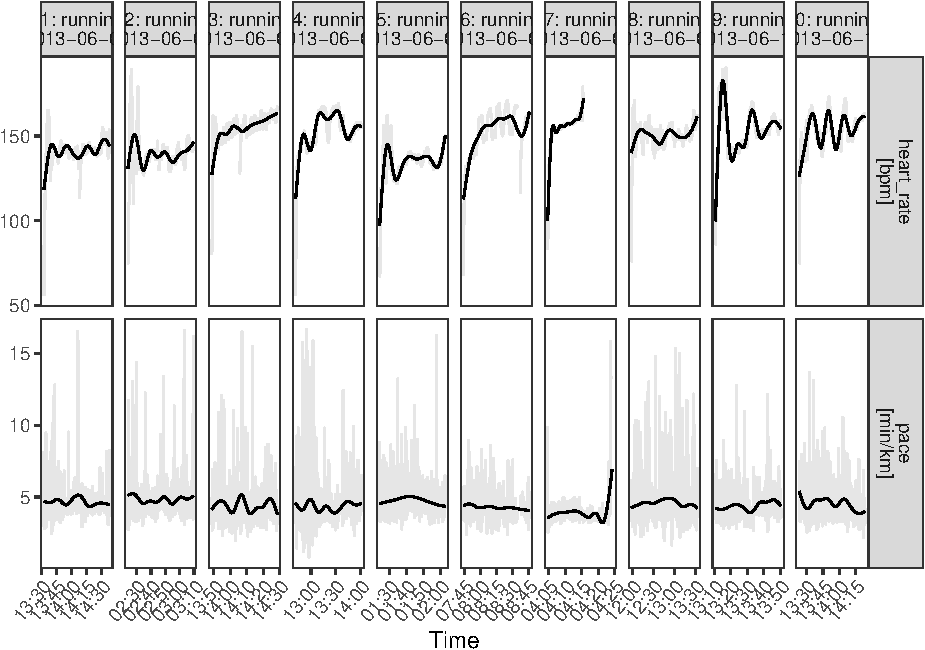
\includegraphics{code4stem_files/figure-latex/unnamed-chunk-4-1.pdf}

but the plot looks better with a wider plotting window.

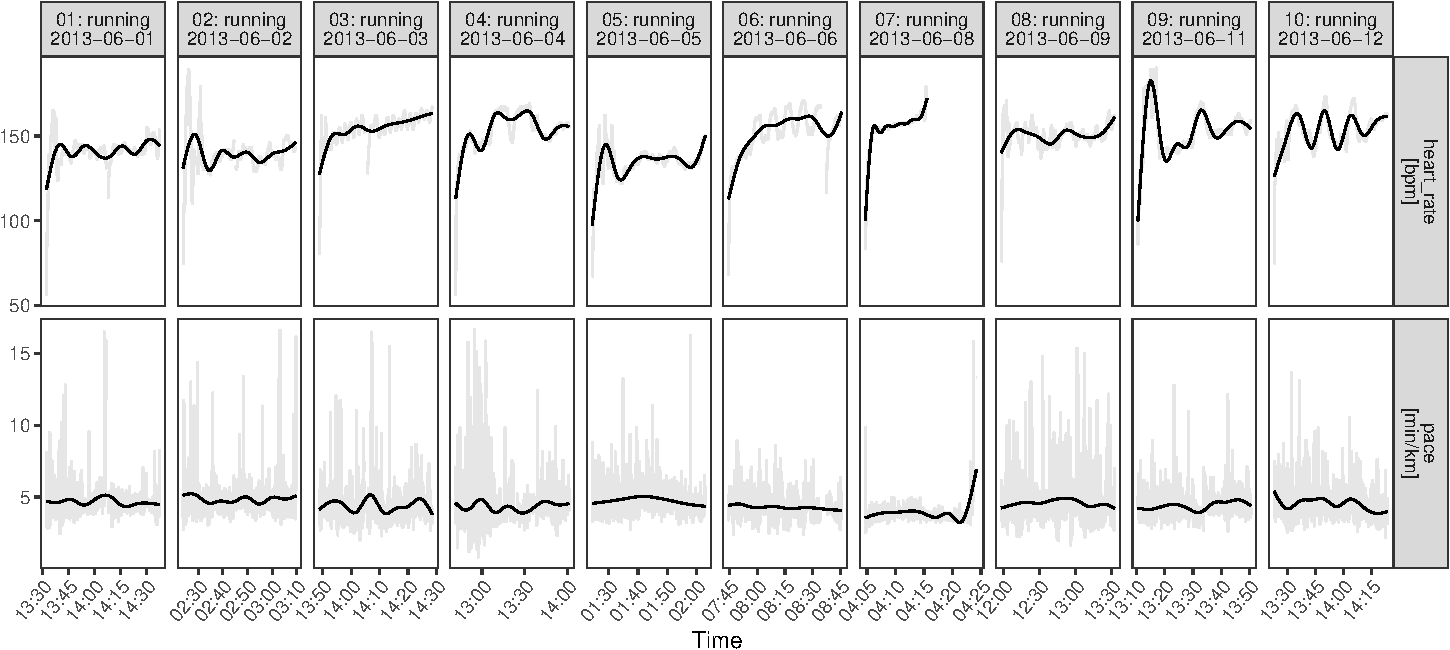
\includegraphics{code4stem_files/figure-latex/unnamed-chunk-5-1.pdf}

\hypertarget{resources}{%
\section{Resources}\label{resources}}

\begin{itemize}
\tightlist
\item
  \href{http://daringfireball.net/projects/markdown/}{Markdown main page}
\item
  \href{http://rmarkdown.rstudio.com/}{R Markdown}
\item
  \href{http://kbroman.org/knitr_knutshell/}{knitr in a nutshell} tutorial by Karl Broman
\end{itemize}

\hypertarget{useful-r-functions-examples}{%
\chapter{Useful R Functions + Examples}\label{useful-r-functions-examples}}

\begin{quote}
This is \emph{NOT} intended to be fully comprehensive list of every useful R function that exists, but is a practical demonstration of selected relevant examples presented in user-friendly format, all available in base R. For a wider collection to work through, this Reference Card is recommended: \url{https://cran.r-project.org/doc/contrib/Baggott-refcard-v2.pdf}
\end{quote}

\begin{quote}
Additional CRAN reference cards and R guides (including non-English documentation) found here: \url{https://cran.r-project.org/other-docs.html}
\end{quote}

\hypertarget{contents}{%
\section{Contents}\label{contents}}

A. Essentials\\
* 1. \texttt{getwd()}, \texttt{setwd()}\\
* 2. \texttt{?foo}, \texttt{help(foo)}, \texttt{example(foo)}\\
* 3. \texttt{install.packages("foo")}, \texttt{library("foo")}\\
* 4. \texttt{devtools::install\_github("username/packagename")}\\
* 5. \texttt{data("foo")}\\
* 6. \texttt{read.csv}, \texttt{read.table}\\
* 7. \texttt{write.table()}\\
* 8. \texttt{save()}, \texttt{load()}

B. Basics\\
* 9. \texttt{c()}, \texttt{cbind()}, \texttt{rbind()}, \texttt{matrix()}\\
* 10. \texttt{length()}, \texttt{dim()}\\
* 11. \texttt{sort()}, \texttt{\textquotesingle{}vector\textquotesingle{}{[}{]}}, \texttt{\textquotesingle{}matrix\textquotesingle{}{[}{]}}\\
* 12. \texttt{data.frame()}, \texttt{class()}, \texttt{names()}, \texttt{str()}, \texttt{summary()}, \texttt{View()}, \texttt{head()}, \texttt{tail()}, \texttt{as.data.frame()}

C. Core\\
* 13. \texttt{df{[}order(),{]}}\\
* 14. \texttt{df{[},c(){]}}, \texttt{df{[}which(),{]}}\\
* 15. \texttt{table()}\\
* 16. \texttt{mean()}, \texttt{median()}, \texttt{sd()}, \texttt{var()}, \texttt{sum()}, \texttt{min()}, \texttt{max()}, \texttt{range()}\\
* 17. \texttt{apply()}\\
* 18. \texttt{lapply()} using \texttt{list()}\\
* 19. \texttt{tapply()}

D. Common\\
* 20. \texttt{if} statement, \texttt{if...else} statement\\
* 21. \texttt{for} loop\\
* 22. \texttt{function()...}

\hypertarget{r-syntax}{%
\section{R Syntax}\label{r-syntax}}

\emph{REMEMBER: KEY R LANGUAGE SYNTAX}

\begin{itemize}
\tightlist
\item
  \textbf{Case Sensitivity}: as per most UNIX-based packages, R is case sensitive, hence \texttt{X} and \texttt{x} are different symbols and would refer to different variables.\\
\item
  \textbf{Expressions vs Assignments}: an expression, like \texttt{3\ +\ 5} can be given as a command which will be evaluated and the value immediately printed, but not stored. An assignment however, like \texttt{sum\ \textless{}-\ 3\ +\ 5} using the assignment operator \texttt{\textless{}-} also evaluates the expression \texttt{3\ +\ 5}, but instead of printing and not storing, it stores the value in the object \texttt{sum} but doesn't print the result. The object \texttt{sum} would need to be called to print the result.\\
\item
  \textbf{Reserved Words}: choice for naming objects is almost entirely free, except for these reserved words: \url{https://stat.ethz.ch/R-manual/R-devel/library/base/html/Reserved.html}\\
\item
  \textbf{Spacing}: outside of the function structure, spaces don't matter, e.g. \texttt{3+5} is the same as \texttt{3+\ \ \ \ \ 5} is the same as \texttt{3\ +\ 5}. For more best-practices for R code Hadley Wickham's Style Guide is a useful reference: \url{http://adv-r.had.co.nz/Style.html}
\item
  \textbf{Comments}: add comments within your code using a hastag, \texttt{\#}. R will ignore everything to the right of the hashtag within that line
\end{itemize}

\hypertarget{functional-examples}{%
\section{Functional examples}\label{functional-examples}}

\begin{enumerate}
\def\labelenumi{\arabic{enumi}.}
\tightlist
\item
  Working Directory management
\end{enumerate}

\begin{itemize}
\tightlist
\item
  \texttt{getwd()}, \texttt{setwd()}
  R/RStudio is always pointed at a specific directory on your computer, so it's important to be able to check what's the current directory using \texttt{getwd()}, and to be able to change and specify a different directory to work in using \texttt{setwd()}.
\end{itemize}

\#check the directory R is currently pointed at
getwd()

\begin{enumerate}
\def\labelenumi{\arabic{enumi}.}
\setcounter{enumi}{1}
\tightlist
\item
  Bring up help documentation \& examples
\end{enumerate}

\begin{itemize}
\tightlist
\item
  \texttt{?foo}, \texttt{help(foo)}, \texttt{example(foo)}
\end{itemize}

\begin{Shaded}
\begin{Highlighting}[]
\NormalTok{?boxplot}
\KeywordTok{help}\NormalTok{(boxplot)}
\KeywordTok{example}\NormalTok{(boxplot)}
\end{Highlighting}
\end{Shaded}

\begin{center}\rule{0.5\linewidth}{0.5pt}\end{center}

\begin{enumerate}
\def\labelenumi{\arabic{enumi}.}
\setcounter{enumi}{2}
\tightlist
\item
  Load \& Call CRAN Packages
\end{enumerate}

\begin{itemize}
\tightlist
\item
  \texttt{install.packages("foo")}, \texttt{library("foo")}
  Packages are add-on functionality built for R but not pre-installed (base R), hence you need to install/load the packages you want yourself. The majority of packages you'd want have been submitted to and are available via CRAN. At time of writing, the CRAN package repository featured 8,592 available packages.
\end{itemize}

\begin{enumerate}
\def\labelenumi{\arabic{enumi}.}
\setcounter{enumi}{3}
\tightlist
\item
  Load \& Call Packages from GitHub
\end{enumerate}

\begin{itemize}
\tightlist
\item
  \texttt{devtools::install\_github("username/packagename")}
  Not all packages you'll want will be available via CRAN, and you'll likely need to get certain packages from GitHub accounts. This example shows how to install the \texttt{shinyapps} package from RStudio's GitHub account.
\item
  install.packages(``devtools'') \#pre-requisite for \texttt{devtools...} function
\item
  devtools::install\_github(``rstudio/shinyapps'') \#install specific package from specific GitHub account
\item
  library(``shinyapps'') \#Call package
\end{itemize}

\begin{enumerate}
\def\labelenumi{\arabic{enumi}.}
\setcounter{enumi}{4}
\tightlist
\item
  Load datasets from base R \& Loaded Packages
\end{enumerate}

\begin{itemize}
\tightlist
\item
  \texttt{data("foo")}
\end{itemize}

\begin{Shaded}
\begin{Highlighting}[]
\CommentTok{#AIM: show available datasets}
\KeywordTok{data}\NormalTok{() }

\CommentTok{#AIM: load an available dataset}
\KeywordTok{data}\NormalTok{(}\StringTok{"iris"}\NormalTok{) }
\end{Highlighting}
\end{Shaded}

\begin{center}\rule{0.5\linewidth}{0.5pt}\end{center}

\begin{enumerate}
\def\labelenumi{\arabic{enumi}.}
\setcounter{enumi}{5}
\tightlist
\item
  I/O Loading Existing Local Data
\end{enumerate}

\begin{itemize}
\tightlist
\item
  \texttt{read.csv}, \texttt{read.table}
\end{itemize}

\begin{enumerate}
\def\labelenumi{(\alph{enumi})}
\tightlist
\item
  I/O When already in the working directory where the data is
\end{enumerate}

Import a local \textbf{csv} file (i.e.~where data is separated by \textbf{commas}), saving it as an object:
- object \textless{}- read.csv(``xxx.csv'')

Import a local tab delimited file (i.e.~where data is separated by \textbf{tabs}), saving it as an object:
- object \textless{}- read.csv(``xxx.csv'', header = FALSE)
---

\begin{enumerate}
\def\labelenumi{(\alph{enumi})}
\setcounter{enumi}{1}
\tightlist
\item
  I/O When NOT in the working directory where the data is
\end{enumerate}

For example to import and save a local \textbf{csv} file from a different working directory you either need to specify the file path (operating system specific), e.g.:

on a mac:
- object \textless{}- read.csv(``\textasciitilde{}/Desktop/R/data.csv'')

on windows:
= object \textless{}- read.csv(``C:/Desktop/R/data.csv'')

OR

You can use the file.choose() command which will interactively open up the file dialog box for you to browse and select the local file, e.g.:
- object \textless{}- read.csv(file.choose())

\begin{enumerate}
\def\labelenumi{(\alph{enumi})}
\setcounter{enumi}{2}
\tightlist
\item
  I/O Copying \& Pasting Data
\end{enumerate}

For relatively small amounts of data you can do an equivalent copy paste (operating system specific):

on a mac:
- object \textless{}- read.table(pipe(``pbpaste''))

on windows:
- object \textless{}- read.table(file = ``clipboard'')

\begin{enumerate}
\def\labelenumi{(\alph{enumi})}
\setcounter{enumi}{3}
\tightlist
\item
  I/O Loading Non-Numerical Data - character strings
\end{enumerate}

Be careful when loading text data! R may assume character strings are statistical factor variables, e.g. ``low'', ``medium'', ``high'', when are just individual labels like names. To specify text data NOT to be converted into factor variables, add \texttt{stringsAsFactor\ =\ FALSE} to your \texttt{read.csv/read.table} command:
- object \textless{}- read.table(``xxx.txt'', stringsAsFactors = FALSE)

\begin{enumerate}
\def\labelenumi{(\alph{enumi})}
\setcounter{enumi}{4}
\tightlist
\item
  I/O Downloading Remote Data
\end{enumerate}

For accessing files from the web you can use the same \texttt{read.csv/read.table} commands. However, the file being downloaded does need to be in an R-friendly format (maximum of 1 header row, subsequent rows are the equivalent of one data record per row, no extraneous footnotes etc.). Here is an example downloading an online csv file of coffee harvest data used in a Nature study:
- object \textless{}- read.csv(``\url{http://sumsar.net/files/posts/2014-02-04-bayesian-first-aid-one-sample-t-test/roubik_2002_coffe_yield.csv}'')

\begin{enumerate}
\def\labelenumi{\arabic{enumi}.}
\setcounter{enumi}{6}
\tightlist
\item
  I/O Exporting Data Frame
\end{enumerate}

\begin{itemize}
\tightlist
\item
  \texttt{write.table()}
\end{itemize}

Navigate to the working directory you want to save the data table into, then run the command (in this case creating a tab delimited file):
- write.table(object, ``xxx.txt'', sep = "\t")

\begin{enumerate}
\def\labelenumi{\arabic{enumi}.}
\setcounter{enumi}{7}
\tightlist
\item
  I/O Saving Down \& Loading Objects
\end{enumerate}

\begin{itemize}
\tightlist
\item
  \texttt{save()}, \texttt{load()}
\end{itemize}

These two commands allow you to save a named R object to a file and restore that object again.\\
Navigate to the working directory you want to save the object in then run the command:
- save(object, file = ``xxx.rda'')

reload the object:
- load(``xxx.rda'')

\begin{enumerate}
\def\labelenumi{\arabic{enumi}.}
\setcounter{enumi}{8}
\tightlist
\item
  Vector \& Matrix Construction
\end{enumerate}

\begin{itemize}
\tightlist
\item
  \texttt{c()}, \texttt{cbind()}, \texttt{rbind()}, \texttt{matrix()}
  Vectors (lists) \& Matrices (two-dimensional arrays) are very common R data structures.
\end{itemize}

\begin{Shaded}
\begin{Highlighting}[]
\CommentTok{#use c() to construct a vector by concatenating data}
\NormalTok{foo <-}\StringTok{ }\KeywordTok{c}\NormalTok{(}\DecValTok{1}\NormalTok{, }\DecValTok{2}\NormalTok{, }\DecValTok{3}\NormalTok{, }\DecValTok{4}\NormalTok{) }\CommentTok{#example of a numeric vector}
\NormalTok{oof <-}\StringTok{ }\KeywordTok{c}\NormalTok{(}\StringTok{"A"}\NormalTok{, }\StringTok{"B"}\NormalTok{, }\StringTok{"C"}\NormalTok{, }\StringTok{"D"}\NormalTok{) }\CommentTok{#example of a character vector}
\NormalTok{ofo <-}\StringTok{ }\KeywordTok{c}\NormalTok{(}\OtherTok{TRUE}\NormalTok{, }\OtherTok{FALSE}\NormalTok{, }\OtherTok{TRUE}\NormalTok{, }\OtherTok{TRUE}\NormalTok{) }\CommentTok{#example of a logical vector}

\CommentTok{#use cbind() & rbind() to construct matrices}
\NormalTok{coof <-}\StringTok{ }\KeywordTok{cbind}\NormalTok{(foo, oof) }\CommentTok{#bind vectors in column concatenation to make a matrix}
\NormalTok{roof <-}\StringTok{ }\KeywordTok{rbind}\NormalTok{(foo, oof) }\CommentTok{#bind vectors in row concatenation to make a matrix}

\CommentTok{#use matrix() to construct matrices}
\NormalTok{moof <-}\StringTok{ }\KeywordTok{matrix}\NormalTok{(}\DataTypeTok{data =} \DecValTok{1}\OperatorTok{:}\DecValTok{12}\NormalTok{, }\DataTypeTok{nrow=}\DecValTok{3}\NormalTok{, }\DataTypeTok{ncol=}\DecValTok{4}\NormalTok{) }\CommentTok{#creates matrix by specifying set of values, no. of rows & no. of columns}
\end{Highlighting}
\end{Shaded}

\begin{enumerate}
\def\labelenumi{\arabic{enumi}.}
\setcounter{enumi}{9}
\tightlist
\item
  Vector \& Matrix Explore
\end{enumerate}

\begin{itemize}
\tightlist
\item
  \texttt{length()}, \texttt{dim()}
\end{itemize}

\begin{Shaded}
\begin{Highlighting}[]
\KeywordTok{length}\NormalTok{(foo) }\CommentTok{#length of vector}

\KeywordTok{dim}\NormalTok{(coof) }\CommentTok{#returns dimensions (no. of rows & columns) of vector/matrix/dataframe}
\end{Highlighting}
\end{Shaded}

\begin{enumerate}
\def\labelenumi{\arabic{enumi}.}
\setcounter{enumi}{10}
\tightlist
\item
  Vector \& Matrix Sort \& Select
\end{enumerate}

\begin{itemize}
\tightlist
\item
  \texttt{sort()}, \texttt{\textquotesingle{}vector\textquotesingle{}{[}{]}}, \texttt{\textquotesingle{}matrix\textquotesingle{}{[}{]}}
\end{itemize}

\begin{Shaded}
\begin{Highlighting}[]
\CommentTok{#create another numeric vector}
\NormalTok{jumble <-}\StringTok{ }\KeywordTok{c}\NormalTok{(}\DecValTok{4}\NormalTok{, }\DecValTok{1}\NormalTok{, }\DecValTok{2}\NormalTok{, }\DecValTok{3}\NormalTok{)}
\KeywordTok{sort}\NormalTok{(jumble) }\CommentTok{#sorts a numeric vector in ascending order (default)}
\KeywordTok{sort}\NormalTok{(jumble, }\DataTypeTok{decreasing =} \OtherTok{TRUE}\NormalTok{) }\CommentTok{#specify the decreasing arg to reverse default order}

\CommentTok{#create another character vector}
\NormalTok{mumble <-}\StringTok{ }\KeywordTok{c}\NormalTok{( }\StringTok{"D"}\NormalTok{, }\StringTok{"B"}\NormalTok{, }\StringTok{"C"}\NormalTok{, }\StringTok{"A"}\NormalTok{)}
\KeywordTok{sort}\NormalTok{(mumble) }\CommentTok{#sorts a character vector in alphabetical order (default)}
\KeywordTok{sort}\NormalTok{(mumble, }\DataTypeTok{decreasing =} \OtherTok{TRUE}\NormalTok{) }\CommentTok{#specify the decreasing arg to reverse default order}

\NormalTok{jumble[}\DecValTok{1}\NormalTok{] }\CommentTok{#selects first value in our jumble vector}
\KeywordTok{tail}\NormalTok{(jumble, }\DataTypeTok{n=}\DecValTok{1}\NormalTok{) }\CommentTok{#selects last value}
\NormalTok{jumble[}\KeywordTok{c}\NormalTok{(}\DecValTok{1}\NormalTok{,}\DecValTok{3}\NormalTok{)] }\CommentTok{#selects the 1st & 3rd values}
\NormalTok{jumble[}\OperatorTok{-}\KeywordTok{c}\NormalTok{(}\DecValTok{1}\NormalTok{,}\DecValTok{3}\NormalTok{)] }\CommentTok{#selects everything except the 1st & 3rd values}

\NormalTok{coof[}\DecValTok{1}\NormalTok{,] }\CommentTok{#selects the 1st row of our coof matrix}
\NormalTok{coof[,}\DecValTok{1}\NormalTok{] }\CommentTok{#selects the 1st column}
\NormalTok{coof[}\DecValTok{2}\NormalTok{,}\DecValTok{1}\NormalTok{] }\CommentTok{#selects the value in the 2nd row, 1st column}
\NormalTok{coof[,}\StringTok{"oof"}\NormalTok{] }\CommentTok{#selects the column named "oof"}
\NormalTok{coof[}\DecValTok{1}\OperatorTok{:}\DecValTok{3}\NormalTok{,] }\CommentTok{#selects columns 1 to 3 inclusive}
\NormalTok{coof[}\KeywordTok{c}\NormalTok{(}\DecValTok{1}\NormalTok{,}\DecValTok{2}\NormalTok{,}\DecValTok{3}\NormalTok{),] }\CommentTok{#selects the 1st, 2nd & 3rd rows (same as previous)}
\end{Highlighting}
\end{Shaded}

\begin{enumerate}
\def\labelenumi{\arabic{enumi}.}
\setcounter{enumi}{11}
\tightlist
\item
  Create \& Explore Data Frames
\end{enumerate}

\begin{itemize}
\tightlist
\item
  \texttt{data.frame()}, \texttt{class()}, \texttt{names()}, \texttt{str()}, \texttt{summary()}, \texttt{View()}, \texttt{head()}, \texttt{tail()}, \texttt{as.data.frame()}
  A data frame is a matrix-like data structure made up of lists of variables with the same number of rows, which can be of differing data types (numeric, character, factor etc.) - matrices must have columns all of the same data type.
\end{itemize}

\begin{Shaded}
\begin{Highlighting}[]
\CommentTok{#create a data frame with 3 columns with 4 rows each}
\NormalTok{doof <-}\StringTok{ }\KeywordTok{data.frame}\NormalTok{(}\StringTok{"V1"}\NormalTok{=}\DecValTok{1}\OperatorTok{:}\DecValTok{4}\NormalTok{, }\StringTok{"V2"}\NormalTok{=}\KeywordTok{c}\NormalTok{(}\StringTok{"A"}\NormalTok{,}\StringTok{"B"}\NormalTok{,}\StringTok{"C"}\NormalTok{,}\StringTok{"D"}\NormalTok{), }\StringTok{"V3"}\NormalTok{=}\DecValTok{5}\OperatorTok{:}\DecValTok{8}\NormalTok{)}

\KeywordTok{class}\NormalTok{(doof) }\CommentTok{#check data frame object class}
\KeywordTok{names}\NormalTok{(doof) }\CommentTok{# returns column names}
\KeywordTok{str}\NormalTok{(doof) }\CommentTok{#see structure of data frame}
\KeywordTok{summary}\NormalTok{(doof) }\CommentTok{#returns basic summary stats}
\KeywordTok{View}\NormalTok{(doof) }\CommentTok{#invokes spreadsheet-style viewer}
\KeywordTok{head}\NormalTok{(doof, }\DataTypeTok{n=}\DecValTok{2}\NormalTok{) }\CommentTok{#shows first parts of object, here requesting the first 2 rows}
\KeywordTok{tail}\NormalTok{(doof, }\DataTypeTok{n=}\DecValTok{2}\NormalTok{) }\CommentTok{#shows last parts of object, here requesting the last 2 rows}

\NormalTok{convert <-}\StringTok{ }\KeywordTok{as.data.frame}\NormalTok{(coof) }\CommentTok{#convert a non-data frame object into a data frame}
\end{Highlighting}
\end{Shaded}

\begin{enumerate}
\def\labelenumi{\arabic{enumi}.}
\setcounter{enumi}{12}
\tightlist
\item
  Data Frame Sort
\end{enumerate}

\begin{itemize}
\tightlist
\item
  \texttt{df{[}order(),{]}}
\end{itemize}

\begin{Shaded}
\begin{Highlighting}[]
\CommentTok{#use 'painters' data frame}
\KeywordTok{library}\NormalTok{(}\StringTok{"MASS"}\NormalTok{) }\CommentTok{#call package with the required data}
\KeywordTok{data}\NormalTok{(}\StringTok{"painters"}\NormalTok{) }\CommentTok{#load required data}
\KeywordTok{View}\NormalTok{(painters) }\CommentTok{#scan dataset}

\CommentTok{#syntax for using a specific variable: df=data frame, '$', V1=variable name}
\NormalTok{df}\OperatorTok{$}\NormalTok{V1 }

\CommentTok{#AIM: print the 'School' variable column}
\NormalTok{painters}\OperatorTok{$}\NormalTok{School}

\CommentTok{#syntax for df[order(),]}
\NormalTok{df[}\KeywordTok{order}\NormalTok{(df}\OperatorTok{$}\NormalTok{V1, df}\OperatorTok{$}\NormalTok{V2...),] }\CommentTok{#function arguments: df=data frame, in square brackets specify within the order() the columns with which to sort the ROWS by, where default ordering is Ascending, the tailing comma specifies returning all the columns in the df. If only certain columns are wanted this can be specified after the comma.}

\CommentTok{#AIM: order the dataset rows based on the painters' Composition Score column, in Ascending order}
\NormalTok{painters[}\KeywordTok{order}\NormalTok{(painters}\OperatorTok{$}\NormalTok{Composition),] }\CommentTok{#Composition is the sorting variable}

\CommentTok{#AIM: order the dataset rows based on the painters' Composition Score column, in Descending order}
\NormalTok{painters[}\KeywordTok{order}\NormalTok{(}\OperatorTok{-}\NormalTok{painters}\OperatorTok{$}\NormalTok{Composition),] }\CommentTok{#append a minus sign in front of the variable you want to sort by in Descending order}

\CommentTok{#AIM: order the dataset rows based on the painters' Composition Score column, in Descending order but return just the first 3 columns}
\NormalTok{painters[}\KeywordTok{order}\NormalTok{(}\OperatorTok{-}\NormalTok{painters}\OperatorTok{$}\NormalTok{Composition), }\KeywordTok{c}\NormalTok{(}\DecValTok{1}\OperatorTok{:}\DecValTok{3}\NormalTok{)]}
\end{Highlighting}
\end{Shaded}

\begin{enumerate}
\def\labelenumi{\arabic{enumi}.}
\setcounter{enumi}{13}
\tightlist
\item
  Data Frame Select \& Deselect
\end{enumerate}

\begin{itemize}
\tightlist
\item
  \texttt{df{[},c(){]}}, \texttt{df{[}which(),{]}}
\end{itemize}

\begin{Shaded}
\begin{Highlighting}[]
\CommentTok{#use 'painters' data frame}

\CommentTok{#syntax for select & deselect based on column variables}
\NormalTok{df[, }\KeywordTok{c}\NormalTok{(}\StringTok{"V1"}\NormalTok{, }\StringTok{"V2"}\NormalTok{...)] }\CommentTok{#function arguments: df=data frame, in square brackets specify columns to select or deselect. The comma specifies returning all the rows. If certain rows are wanted this can be specified before the comma.}

\CommentTok{#AIM: select the Composition & Drawing variables based on their column name}
\NormalTok{painters[, }\KeywordTok{c}\NormalTok{(}\StringTok{"Composition"}\NormalTok{, }\StringTok{"Drawing"}\NormalTok{)] }\CommentTok{#subset the df, selecting just the named columns (and all the rows)}

\CommentTok{#AIM: select the Composition & Drawing variables based on their column positions in the painters data frame}
\NormalTok{painters[, }\KeywordTok{c}\NormalTok{(}\DecValTok{1}\NormalTok{,}\DecValTok{2}\NormalTok{)] }\CommentTok{#subset the df, selecting just the 1st & 2nd columns (and all the rows)}

\CommentTok{#AIM: drop the Expression variable based on it's column position in the painters data frame and return just the first 5 rows}
\NormalTok{painters[}\KeywordTok{c}\NormalTok{(}\DecValTok{1}\OperatorTok{:}\DecValTok{5}\NormalTok{), }\DecValTok{-4}\NormalTok{] }\CommentTok{#returns the subsetted df having deselected the 4th column, Expression and the first 5 rows}


\CommentTok{#syntax for select & deselect based on row variable values}
\NormalTok{df[}\KeywordTok{which}\NormalTok{(),] }\CommentTok{#df=data frame, specify the variable value within the `which()` to subset the df on. Again, the tailing comma specifies returning all the columns. If certain columns are wanted this can be specified after the comma.}

\CommentTok{#AIM: select all rows where the painters' School is the 'A' category}
\NormalTok{painters[}\KeywordTok{which}\NormalTok{(painters}\OperatorTok{$}\NormalTok{School }\OperatorTok{==}\StringTok{ "A"}\NormalTok{),] }\CommentTok{#returns the subsetted df where equality holds true, i.e. row value in School variable column is 'A'}

\CommentTok{#AIM: deselect all rows where the painters' School is the 'A' category, i.e. return df subset without 'A' values, AND also only select rows where Colour score > 10}
\NormalTok{painters[}\KeywordTok{which}\NormalTok{(painters}\OperatorTok{$}\NormalTok{School }\OperatorTok{!=}\StringTok{ "A"} \OperatorTok{&}\StringTok{ }\NormalTok{painters}\OperatorTok{$}\NormalTok{Colour }\OperatorTok{>}\StringTok{ }\DecValTok{10}\NormalTok{),] }\CommentTok{#returns the subsetted df where equality holds true, i.e. row value in School variable column is 'not A', AND the Colour score filter is also true.}
\end{Highlighting}
\end{Shaded}

\begin{enumerate}
\def\labelenumi{\arabic{enumi}.}
\setcounter{enumi}{14}
\tightlist
\item
  Data Frame Frequency Calculations
\end{enumerate}

\begin{itemize}
\tightlist
\item
  \texttt{table()}
\end{itemize}

\begin{Shaded}
\begin{Highlighting}[]
\CommentTok{#create new data frame}
\NormalTok{flavour <-}\StringTok{ }\KeywordTok{c}\NormalTok{(}\StringTok{"choc"}\NormalTok{, }\StringTok{"strawberry"}\NormalTok{, }\StringTok{"vanilla"}\NormalTok{, }\StringTok{"choc"}\NormalTok{, }\StringTok{"strawberry"}\NormalTok{, }\StringTok{"strawberry"}\NormalTok{) }
\NormalTok{gender <-}\StringTok{ }\KeywordTok{c}\NormalTok{(}\StringTok{"F"}\NormalTok{, }\StringTok{"F"}\NormalTok{, }\StringTok{"M"}\NormalTok{, }\StringTok{"M"}\NormalTok{, }\StringTok{"F"}\NormalTok{, }\StringTok{"M"}\NormalTok{)}
\NormalTok{icecream <-}\StringTok{ }\KeywordTok{data.frame}\NormalTok{(flavour, gender) }\CommentTok{#icecream df made up of 2 factor variables, flavour & gender, with 3 & 2 levels respectively (choc/strawberry/vanilla & F/M)}

\CommentTok{#AIM: create a frequency distribution table which shows the count of each gender in the df}
\KeywordTok{table}\NormalTok{(icecream}\OperatorTok{$}\NormalTok{gender) }

\CommentTok{#AIM: create a frequency distribution table which shows the count of each flavour in the df}
\KeywordTok{table}\NormalTok{(icecream}\OperatorTok{$}\NormalTok{flavour)}

\CommentTok{#AIM: create Contingency/2-Way Table showing the counts for each combination of flavour & gender level }
\KeywordTok{table}\NormalTok{(icecream}\OperatorTok{$}\NormalTok{flavour, icecream}\OperatorTok{$}\NormalTok{gender)}
\end{Highlighting}
\end{Shaded}

\begin{enumerate}
\def\labelenumi{\arabic{enumi}.}
\setcounter{enumi}{15}
\tightlist
\item
  Descriptive/Summary Stats Functions
\end{enumerate}

\begin{itemize}
\tightlist
\item
  \texttt{mean()}, \texttt{median()}, \texttt{sd()}, \texttt{var()}, \texttt{sum()}, \texttt{min()}, \texttt{max()}, \texttt{range()}
\end{itemize}

\begin{Shaded}
\begin{Highlighting}[]
\CommentTok{#re-using the jumble vector from before}
\NormalTok{jumble <-}\StringTok{ }\KeywordTok{c}\NormalTok{(}\DecValTok{4}\NormalTok{, }\DecValTok{1}\NormalTok{, }\DecValTok{2}\NormalTok{, }\DecValTok{3}\NormalTok{) }

\KeywordTok{mean}\NormalTok{(jumble)}
\KeywordTok{median}\NormalTok{(jumble)}
\KeywordTok{sd}\NormalTok{(jumble)}
\KeywordTok{var}\NormalTok{(jumble)}
\KeywordTok{sum}\NormalTok{(jumble)}
\KeywordTok{min}\NormalTok{(jumble)}
\KeywordTok{max}\NormalTok{(jumble)}
\KeywordTok{range}\NormalTok{(jumble)}
\end{Highlighting}
\end{Shaded}

\begin{enumerate}
\def\labelenumi{\arabic{enumi}.}
\setcounter{enumi}{16}
\tightlist
\item
  Apply Functions
\end{enumerate}

\begin{itemize}
\tightlist
\item
  \texttt{apply()}
  \texttt{apply()} returns a vector, array or list of values where a specified function has been applied to the `margins' (rows/cols combo) of the original vector/array/list.
\end{itemize}

\begin{Shaded}
\begin{Highlighting}[]
\CommentTok{#re-using the moof matrix from before}
\NormalTok{moof <-}\StringTok{ }\KeywordTok{matrix}\NormalTok{(}\DataTypeTok{data =} \DecValTok{1}\OperatorTok{:}\DecValTok{12}\NormalTok{, }\DataTypeTok{nrow=}\DecValTok{3}\NormalTok{, }\DataTypeTok{ncol=}\DecValTok{4}\NormalTok{) }

\CommentTok{#apply syntax}
\KeywordTok{apply}\NormalTok{(X, MARGIN, FUN,...) }\CommentTok{#function arguments: X=an array, MARGIN=1 to apply to rows/2 to apply to cols, FUN=function to apply}

\CommentTok{#AIM: using the moof matrix, apply the sum function to the rows}
\KeywordTok{apply}\NormalTok{(moof, }\DecValTok{1}\NormalTok{, sum) }

\CommentTok{#AIM: using the moof matrix, apply the sum function to the columns}
\KeywordTok{apply}\NormalTok{(moof, }\DecValTok{2}\NormalTok{, sum) }
\end{Highlighting}
\end{Shaded}

\begin{enumerate}
\def\labelenumi{\arabic{enumi}.}
\setcounter{enumi}{17}
\tightlist
\item
  Apply Functions
\end{enumerate}

\begin{itemize}
\tightlist
\item
  \texttt{lapply()} using \texttt{list()}
  A list, a common data structure, is a generic vector containing objects of any types.
  \texttt{lapply()} returns a list where each element returned is the result of applying a specified function to the objects in the list.
\end{itemize}

\begin{Shaded}
\begin{Highlighting}[]
\CommentTok{#create list of various vectors and matrices}
\NormalTok{bundle <-}\StringTok{ }\KeywordTok{list}\NormalTok{(moof, jumble, foo) }

\CommentTok{#lapply syntax}
\KeywordTok{lapply}\NormalTok{(X, FUN,...) }\CommentTok{#function arguments: X=a list, FUN=function to apply}

\CommentTok{#AIM: using the bundle list, apply the mean function to each object in the list}
\KeywordTok{lapply}\NormalTok{(bundle, mean)}
\end{Highlighting}
\end{Shaded}

\begin{enumerate}
\def\labelenumi{\arabic{enumi}.}
\setcounter{enumi}{18}
\tightlist
\item
  Apply Functions
\end{enumerate}

\begin{itemize}
\tightlist
\item
  \texttt{tapply()}
  \texttt{tapply()} applies a specified function to specified groups/subsets of a factor variable.
\end{itemize}

\begin{Shaded}
\begin{Highlighting}[]
\CommentTok{#tapply syntax}
\KeywordTok{tapply}\NormalTok{(X, INDEX, FUN,...) }\CommentTok{#function arguments: X=an atomic object, INDEX=list of 1+ factors of X length, FUN=function to apply}

\CommentTok{#AIM: calculate the mean Drawing Score of the painters, but grouped by School category}
\KeywordTok{tapply}\NormalTok{(painters}\OperatorTok{$}\NormalTok{Drawing, painters}\OperatorTok{$}\NormalTok{School, mean) }\CommentTok{#grouping the data by the 8 different Schools, apply the mean function to the Drawing Score variable to return the 8 mean scores}
\end{Highlighting}
\end{Shaded}

\begin{enumerate}
\def\labelenumi{\arabic{enumi}.}
\setcounter{enumi}{19}
\tightlist
\item
  Programming Tools
\end{enumerate}

\begin{itemize}
\tightlist
\item
  \texttt{if} statement, \texttt{if...else} statement
  An \texttt{if} statement is used when certain computations are conditional and only execute when a specific condition is met - if the condition is not met, nothing executes. The \texttt{if...else} statement extends the \texttt{if} statement by adding on a computation to execute when the condition is not met, i.e.~the `else' part of the statement.
\end{itemize}

\begin{Shaded}
\begin{Highlighting}[]
\CommentTok{#if-statement syntax}
\ControlFlowTok{if}\NormalTok{ (}\StringTok{'test expression'}\NormalTok{)}
\NormalTok{    \{}
    \StringTok{'statement'}
\NormalTok{    \}}

\CommentTok{#if...else statement}
\ControlFlowTok{if}\NormalTok{ (}\StringTok{'test expression'}\NormalTok{)}
\NormalTok{    \{}
    \StringTok{'statement'}
\NormalTok{    \}}\ControlFlowTok{else}\NormalTok{\{}
    \StringTok{'another statement'}
\NormalTok{    \}}

\CommentTok{#AIM: here we want to test if the object, 'condition_to_test' is smaller than 10. If it is smaller, another object, 'result_after_test' is assigned the value 'smaller'. Otherwise, the 'result_after_test' object is assigned the value 'bigger'}

\CommentTok{#specify the 'test expression'}
\NormalTok{condition_to_test <-}\StringTok{ }\DecValTok{7} 

\CommentTok{#write your 'if...else' function based on a 'statement' or 'another statement' dependent on the 'condition_to_test'. }
\ControlFlowTok{if}\NormalTok{ (condition_to_test }\OperatorTok{>}\StringTok{ }\DecValTok{5}\NormalTok{)}
\NormalTok{    \{}
\NormalTok{    result_after_test =}\StringTok{ 'Above Average'}
\NormalTok{    \}}\ControlFlowTok{else}\NormalTok{\{}
\NormalTok{    result_after_test =}\StringTok{ 'Below Average'}
\NormalTok{    \}}

\CommentTok{#call the resulting 'statement' as per the instruction of the 'if...else' statement}
\NormalTok{result_after_test }
\end{Highlighting}
\end{Shaded}

\begin{enumerate}
\def\labelenumi{\arabic{enumi}.}
\setcounter{enumi}{20}
\tightlist
\item
  Programming Tools
\end{enumerate}

\begin{itemize}
\tightlist
\item
  \texttt{for} loop
  A \texttt{for} loop is an automation method for repeating (looping) a specific set of instructions for each element in a vector.
\end{itemize}

\begin{Shaded}
\begin{Highlighting}[]
\CommentTok{#for loop syntax requires a counter, often called 'i' to denote an index}
\ControlFlowTok{for}\NormalTok{ (}\StringTok{'counter'} \ControlFlowTok{in} \StringTok{'looping vector'}\NormalTok{)}
\NormalTok{    \{}
    \StringTok{'instructions'}
\NormalTok{    \}}

\CommentTok{#AIM: here we want to print the phrase "In the Year yyyy" 6x, once for each year between 2010 to 2015.}
\CommentTok{#this for loop executes the code chunk 'print(past("In the Year", i)) for each of the 'i' index values}
\ControlFlowTok{for}\NormalTok{ (i }\ControlFlowTok{in} \DecValTok{2010}\OperatorTok{:}\DecValTok{2015}\NormalTok{)}
\NormalTok{    \{}
    \KeywordTok{print}\NormalTok{(}\KeywordTok{paste}\NormalTok{(}\StringTok{"In the Year"}\NormalTok{, i))}
\NormalTok{    \}}

\CommentTok{#AIM: create an object which contains 10 items, namely each number between 1 and 10 squared}
\CommentTok{#to store rather than just print results, an empty storage container needs to be created prior to running the loop, here called container}
\NormalTok{container <-}\StringTok{ }\OtherTok{NULL}
\ControlFlowTok{for}\NormalTok{ (i }\ControlFlowTok{in} \DecValTok{1}\OperatorTok{:}\DecValTok{10}\NormalTok{)}
\NormalTok{    \{}
\NormalTok{    container[i] =}\StringTok{ }\NormalTok{i}\OperatorTok{^}\DecValTok{2}
\NormalTok{    \}}

\NormalTok{container }\CommentTok{#check results: the loop is instructed to square every element of the looping vector, 1:10. The ith element returned is therefore the value of i^2, e.g. the 3rd element is 3^2.}
\end{Highlighting}
\end{Shaded}

\begin{enumerate}
\def\labelenumi{\arabic{enumi}.}
\setcounter{enumi}{21}
\tightlist
\item
  Programming Tools
\end{enumerate}

\begin{itemize}
\tightlist
\item
  \texttt{function()...}
  User-programmed functions allow you to specify customised arguments and returned values.
\end{itemize}

\begin{Shaded}
\begin{Highlighting}[]
\CommentTok{#AIM: to create a simplified take-home pay calculator (single-band), called 'takehome_pay'. Our function therefore uses two arguments, a 'tax_rate', and an 'income' level. The code in the curly braces \{\} instructs what the 'takehome_pay' function should do when it is called, namely, calculate the tax owed in an object 'tax', and then return the result of the 'income' object minus the 'tax' object}
\NormalTok{takehome_pay <-}\StringTok{ }\ControlFlowTok{function}\NormalTok{(tax_rate, income)}
\NormalTok{    \{}
\NormalTok{    tax =}\StringTok{ }\NormalTok{tax_rate }\OperatorTok{*}\StringTok{ }\NormalTok{income}
    \KeywordTok{return}\NormalTok{(income }\OperatorTok{-}\StringTok{ }\NormalTok{tax)}
\NormalTok{    \}}

\KeywordTok{takehome_pay}\NormalTok{(}\DataTypeTok{tax_rate =} \FloatTok{0.2}\NormalTok{, }\DataTypeTok{income =} \DecValTok{25000}\NormalTok{) }\CommentTok{#call our function to calculate 'takehome_pay' on a 'tax_rate' of 20% and an 'income' of 25k}
\end{Highlighting}
\end{Shaded}

\begin{enumerate}
\def\labelenumi{\arabic{enumi}.}
\setcounter{enumi}{22}
\tightlist
\item
  Strings\\
\end{enumerate}

\begin{itemize}
\tightlist
\item
  \texttt{grep()}, \texttt{tolower()}, \texttt{nchar()}
\end{itemize}

\begin{enumerate}
\def\labelenumi{\arabic{enumi}.}
\setcounter{enumi}{23}
\tightlist
\item
  Further Data Selection\\
\end{enumerate}

\begin{itemize}
\tightlist
\item
  \texttt{quantile()}, \texttt{cut()}, \texttt{which()}, \texttt{na.omit()}, \texttt{complete.cases()}, \texttt{sample()}
\end{itemize}

\begin{enumerate}
\def\labelenumi{\arabic{enumi}.}
\setcounter{enumi}{24}
\tightlist
\item
  Further Data Creation\\
\end{enumerate}

\begin{itemize}
\tightlist
\item
  \texttt{seq()}, \texttt{rep()}
\end{itemize}

\begin{enumerate}
\def\labelenumi{\arabic{enumi}.}
\setcounter{enumi}{25}
\tightlist
\item
  Other Apply-related functions\\
\end{enumerate}

\begin{itemize}
\tightlist
\item
  \texttt{split()}, \texttt{sapply()}, \texttt{aggregate()}
\end{itemize}

\begin{enumerate}
\def\labelenumi{\arabic{enumi}.}
\setcounter{enumi}{26}
\tightlist
\item
  More Loops\\
\end{enumerate}

\begin{itemize}
\tightlist
\item
  \texttt{while} loop, \texttt{repeat} loop
\end{itemize}

\ldots{}..Ad Infinitum!!

\hypertarget{demo-for-dplyr}{%
\chapter{Demo for dplyr}\label{demo-for-dplyr}}

\begin{Shaded}
\begin{Highlighting}[]
\CommentTok{# Load data and dependencies:}
\KeywordTok{library}\NormalTok{(dplyr)}

\KeywordTok{data}\NormalTok{(iris)}
\end{Highlighting}
\end{Shaded}

Explore the iris data

\begin{Shaded}
\begin{Highlighting}[]
\KeywordTok{head}\NormalTok{(iris)}
\KeywordTok{pairs}\NormalTok{(iris)}
\KeywordTok{str}\NormalTok{(iris)}
\KeywordTok{summary}\NormalTok{(iris)}
\end{Highlighting}
\end{Shaded}

A. \textbf{Select}: keeps only the variables you mention

\begin{Shaded}
\begin{Highlighting}[]
\KeywordTok{select}\NormalTok{(iris, }\DecValTok{1}\OperatorTok{:}\DecValTok{3}\NormalTok{)}
\KeywordTok{select}\NormalTok{(iris, Petal.Width, Species)}
\KeywordTok{select}\NormalTok{(iris, }\KeywordTok{contains}\NormalTok{(}\StringTok{"Petal.Width"}\NormalTok{))}
\KeywordTok{select}\NormalTok{(iris, }\KeywordTok{starts_with}\NormalTok{(}\StringTok{"Species"}\NormalTok{))}
\end{Highlighting}
\end{Shaded}

B. \textbf{Arrange}: sort a variable in descending order

\begin{Shaded}
\begin{Highlighting}[]
\KeywordTok{arrange}\NormalTok{(iris, Sepal.Length)}
\KeywordTok{arrange}\NormalTok{(iris, }\KeywordTok{desc}\NormalTok{(Sepal.Length))}
\KeywordTok{arrange}\NormalTok{(iris, Sepal.Length, }\KeywordTok{desc}\NormalTok{(Sepal.Width))}
\end{Highlighting}
\end{Shaded}

C. \textbf{Filter}: find rows/cases where conditions are true
Note: rows where the condition evaluates to NA are dropped

\begin{Shaded}
\begin{Highlighting}[]
\KeywordTok{filter}\NormalTok{(iris, Petal.Length }\OperatorTok{>}\StringTok{ }\DecValTok{5}\NormalTok{)}
\KeywordTok{filter}\NormalTok{(iris, Petal.Length }\OperatorTok{>}\StringTok{ }\DecValTok{5} \OperatorTok{&}\StringTok{ }\NormalTok{Species }\OperatorTok{==}\StringTok{ "setosa"}\NormalTok{)}
\KeywordTok{filter}\NormalTok{(iris, Petal.Length }\OperatorTok{>}\StringTok{ }\DecValTok{5}\NormalTok{, Species }\OperatorTok{==}\StringTok{ "setosa"}\NormalTok{) }\CommentTok{#the comma is a shorthand for &}
\KeywordTok{filter}\NormalTok{(iris, }\OperatorTok{!}\NormalTok{Species }\OperatorTok{==}\StringTok{ "setosa"}\NormalTok{)}
\end{Highlighting}
\end{Shaded}

D. \textbf{Pipe Example with MaggriteR} (ref: Rene Magritte This is not a pipe)
The long Way, before nesting or multiple variables

\begin{Shaded}
\begin{Highlighting}[]
\NormalTok{data1 <-}\StringTok{ }\KeywordTok{filter}\NormalTok{(iris, Petal.Length }\OperatorTok{>}\StringTok{ }\DecValTok{6}\NormalTok{)}
\NormalTok{data2 <-}\StringTok{ }\KeywordTok{select}\NormalTok{(data1, Petal.Length, Species)}
\end{Highlighting}
\end{Shaded}

With \textbf{DPLYR}:

\begin{Shaded}
\begin{Highlighting}[]
\KeywordTok{select}\NormalTok{(}
  \KeywordTok{filter}\NormalTok{(iris, Petal.Length }\OperatorTok{>}\StringTok{ }\DecValTok{6}\NormalTok{),}
\NormalTok{  Petal.Length, Species) }\OperatorTok
\StringTok{  }\KeywordTok{head}\NormalTok{()}
\end{Highlighting}
\end{Shaded}

\begin{verbatim}
##   Petal.Length   Species
## 1          6.6 virginica
## 2          6.3 virginica
## 3          6.1 virginica
## 4          6.7 virginica
## 5          6.9 virginica
## 6          6.7 virginica
\end{verbatim}

Using pipes with the data variable

\begin{Shaded}
\begin{Highlighting}[]
\NormalTok{iris }\OperatorTok
\StringTok{  }\KeywordTok{filter}\NormalTok{(Petal.Length }\OperatorTok{>}\StringTok{ }\DecValTok{6}\NormalTok{) }\OperatorTok
\StringTok{  }\KeywordTok{select}\NormalTok{(Petal.Length, Species) }\OperatorTok
\StringTok{  }\KeywordTok{head}\NormalTok{()}
\end{Highlighting}
\end{Shaded}

\begin{verbatim}
##   Petal.Length   Species
## 1          6.6 virginica
## 2          6.3 virginica
## 3          6.1 virginica
## 4          6.7 virginica
## 5          6.9 virginica
## 6          6.7 virginica
\end{verbatim}

Using the . to specify where the incoming variable will be piped to:
- myFunction(arg1, arg2 = .)

\begin{Shaded}
\begin{Highlighting}[]
\NormalTok{iris }\OperatorTok
\StringTok{  }\KeywordTok{filter}\NormalTok{(., Species }\OperatorTok{==}\StringTok{ "versicolor"}\NormalTok{)}
\end{Highlighting}
\end{Shaded}

Other magrittr examples:

\begin{Shaded}
\begin{Highlighting}[]
\NormalTok{iris }\OperatorTok
\StringTok{  }\KeywordTok{filter}\NormalTok{(Petal.Length }\OperatorTok{>}\StringTok{ }\FloatTok{2.0}\NormalTok{) }\OperatorTok
\StringTok{  }\KeywordTok{select}\NormalTok{(}\DecValTok{1}\OperatorTok{:}\DecValTok{3}\NormalTok{)}

\NormalTok{iris }\OperatorTok
\StringTok{  }\KeywordTok{select}\NormalTok{(}\KeywordTok{contains}\NormalTok{(}\StringTok{"Width"}\NormalTok{)) }\OperatorTok
\StringTok{  }\KeywordTok{arrange}\NormalTok{(Petal.Width) }\OperatorTok
\StringTok{  }\KeywordTok{head}\NormalTok{()}

\NormalTok{iris }\OperatorTok
\StringTok{  }\KeywordTok{filter}\NormalTok{(Petal.Width }\OperatorTok{==}\StringTok{ "versicolor"}\NormalTok{) }\OperatorTok
\StringTok{  }\KeywordTok{arrange}\NormalTok{(}\KeywordTok{desc}\NormalTok{(Sepal.Width))}

\NormalTok{iris }\OperatorTok
\StringTok{  }\KeywordTok{filter}\NormalTok{(Sepal.Width }\OperatorTok{>}\StringTok{ }\DecValTok{1}\NormalTok{) }\OperatorTok
\StringTok{  }\KeywordTok{View}\NormalTok{()}

\NormalTok{iris }\OperatorTok
\StringTok{  }\KeywordTok{filter}\NormalTok{(Petal.Width  }\OperatorTok{==}\StringTok{ }\FloatTok{0.1}\NormalTok{) }\OperatorTok
\StringTok{  }\KeywordTok{select}\NormalTok{(Sepal.Width) }\OperatorTok
\StringTok{  }\KeywordTok{unique}\NormalTok{()}
\end{Highlighting}
\end{Shaded}

a second way to get the unique values:

\begin{Shaded}
\begin{Highlighting}[]
\NormalTok{iris }\OperatorTok
\StringTok{  }\KeywordTok{filter}\NormalTok{(Petal.Width  }\OperatorTok{==}\StringTok{ }\FloatTok{0.1}\NormalTok{) }\OperatorTok
\StringTok{  }\KeywordTok{distinct}\NormalTok{(Sepal.Width)}
\end{Highlighting}
\end{Shaded}

\begin{verbatim}
##   Sepal.Width
## 1         3.1
## 2         3.0
## 3         4.1
## 4         3.6
\end{verbatim}

E. \textbf{Mutate}: adds new variables and preserves existing; transmute() drops existing variables

\begin{Shaded}
\begin{Highlighting}[]
\NormalTok{iris }\OperatorTok
\StringTok{  }\KeywordTok{mutate}\NormalTok{(}\DataTypeTok{highSpecies =}\NormalTok{ Sepal.Width }\OperatorTok{>}\StringTok{ }\DecValTok{6}\NormalTok{) }\OperatorTok
\StringTok{  }\KeywordTok{head}\NormalTok{()}


\NormalTok{iris }\OperatorTok
\StringTok{  }\KeywordTok{mutate}\NormalTok{(}\DataTypeTok{size =}\NormalTok{ Sepal.Width }\OperatorTok{+}\StringTok{ }\NormalTok{Petal.Width) }\OperatorTok
\StringTok{  }\KeywordTok{head}\NormalTok{()}


\NormalTok{iris }\OperatorTok
\StringTok{  }\KeywordTok{mutate}\NormalTok{(}\DataTypeTok{MeanPetal.Width =} \KeywordTok{mean}\NormalTok{(Petal.Width, }\DataTypeTok{na.rm =} \OtherTok{TRUE}\NormalTok{),}
         \DataTypeTok{greaterThanMeanPetal.Width =} \KeywordTok{ifelse}\NormalTok{(Petal.Width }\OperatorTok{>}\StringTok{ }\NormalTok{MeanPetal.Width, }\DecValTok{1}\NormalTok{, }\DecValTok{0}\NormalTok{)) }\OperatorTok
\StringTok{  }\KeywordTok{head}\NormalTok{()}


\NormalTok{iris }\OperatorTok
\StringTok{  }\KeywordTok{mutate}\NormalTok{(}\DataTypeTok{buckets =} \KeywordTok{cut}\NormalTok{(Petal.Width, }\DecValTok{3}\NormalTok{)) }\OperatorTok
\StringTok{  }\KeywordTok{head}\NormalTok{()}


\NormalTok{iris }\OperatorTok
\StringTok{  }\KeywordTok{mutate}\NormalTok{(}\DataTypeTok{Petal.WidthBuckets =} \KeywordTok{case_when}\NormalTok{(Petal.Width }\OperatorTok{<}\StringTok{ }\DecValTok{1} \OperatorTok{~}\StringTok{ "Low"}\NormalTok{,}
\NormalTok{                               Petal.Width }\OperatorTok{>=}\StringTok{ }\DecValTok{2} \OperatorTok{&}\StringTok{ }\NormalTok{Sepal.Width }\OperatorTok{<}\StringTok{ }\DecValTok{3} \OperatorTok{~}\StringTok{ "Med"}\NormalTok{,}
\NormalTok{                               Petal.Width }\OperatorTok{>=}\StringTok{ }\DecValTok{4} \OperatorTok{~}\StringTok{ "High"}\NormalTok{)) }\OperatorTok
\StringTok{  }\KeywordTok{head}\NormalTok{()}
\end{Highlighting}
\end{Shaded}

E. \textbf{Group\_by and Summarise}: used on grouped data created by group\_by().
The output will have one row for each group.

\begin{Shaded}
\begin{Highlighting}[]
\NormalTok{iris }\OperatorTok
\StringTok{  }\KeywordTok{summarise}\NormalTok{(}\DataTypeTok{Petal.WidthMean =} \KeywordTok{mean}\NormalTok{(Petal.Width),}
            \DataTypeTok{Petal.WidthSD =} \KeywordTok{sd}\NormalTok{(Petal.Width))}

\NormalTok{iris }\OperatorTok
\StringTok{  }\KeywordTok{group_by}\NormalTok{(Petal.Width) }\OperatorTok
\StringTok{  }\KeywordTok{mutate}\NormalTok{(}\DataTypeTok{Petal.WidthMean =} \KeywordTok{mean}\NormalTok{(Petal.Width))}

\NormalTok{iris }\OperatorTok
\StringTok{  }\KeywordTok{group_by}\NormalTok{(Petal.Width) }\OperatorTok
\StringTok{  }\KeywordTok{summarise}\NormalTok{(}\DataTypeTok{Petal.WidthMean =} \KeywordTok{mean}\NormalTok{(Petal.Width))}

\NormalTok{iris }\OperatorTok
\StringTok{  }\KeywordTok{group_by}\NormalTok{(Petal.Width, Species) }\OperatorTok
\StringTok{  }\KeywordTok{summarise}\NormalTok{(}\DataTypeTok{count =} \KeywordTok{n}\NormalTok{())}
\end{Highlighting}
\end{Shaded}

F. \textbf{Slice}: Slice does not work with relational databases because they have no intrinsic notion of row order. If you want to perform the equivalent operation, use filter() and row\_number().

\begin{Shaded}
\begin{Highlighting}[]
\NormalTok{iris }\OperatorTok
\StringTok{  }\KeywordTok{slice}\NormalTok{(}\DecValTok{2}\OperatorTok{:}\DecValTok{4}\NormalTok{) }\OperatorTok
\StringTok{  }\KeywordTok{head}\NormalTok{()}
\end{Highlighting}
\end{Shaded}

\begin{verbatim}
##   Sepal.Length Sepal.Width Petal.Length Petal.Width Species
## 1          4.9         3.0          1.4         0.2  setosa
## 2          4.7         3.2          1.3         0.2  setosa
## 3          4.6         3.1          1.5         0.2  setosa
\end{verbatim}

Other verbs within DPLYR: \textbf{Scoped verbs}

\begin{Shaded}
\begin{Highlighting}[]
\CommentTok{# ungroup}
\NormalTok{iris }\OperatorTok
\StringTok{  }\KeywordTok{group_by}\NormalTok{(Petal.Width, Species) }\OperatorTok
\StringTok{  }\KeywordTok{summarise}\NormalTok{(}\DataTypeTok{count =} \KeywordTok{n}\NormalTok{()) }\OperatorTok
\StringTok{  }\KeywordTok{ungroup}\NormalTok{()}

\CommentTok{# Summarise_all}
\NormalTok{iris }\OperatorTok
\StringTok{  }\KeywordTok{select}\NormalTok{(}\DecValTok{1}\OperatorTok{:}\DecValTok{4}\NormalTok{) }\OperatorTok
\StringTok{  }\KeywordTok{summarise_all}\NormalTok{(mean)}


\NormalTok{iris }\OperatorTok
\StringTok{  }\KeywordTok{select}\NormalTok{(}\DecValTok{1}\OperatorTok{:}\DecValTok{4}\NormalTok{) }\OperatorTok
\StringTok{  }\KeywordTok{summarise_all}\NormalTok{(}\KeywordTok{funs}\NormalTok{(mean, min))}


\NormalTok{iris }\OperatorTok
\StringTok{  }\KeywordTok{summarise_all}\NormalTok{(}\OperatorTok{~}\KeywordTok{length}\NormalTok{(}\KeywordTok{unique}\NormalTok{(.)))}

\CommentTok{# summarise_at}
\NormalTok{iris }\OperatorTok
\StringTok{  }\KeywordTok{summarise_at}\NormalTok{(}\KeywordTok{vars}\NormalTok{(}\OperatorTok{-}\NormalTok{Petal.Width), mean)}


\NormalTok{iris }\OperatorTok
\StringTok{  }\KeywordTok{summarise_at}\NormalTok{(}\KeywordTok{vars}\NormalTok{(}\KeywordTok{contains}\NormalTok{(}\StringTok{"Petal.Width"}\NormalTok{)), }\KeywordTok{funs}\NormalTok{(mean, min))}

\CommentTok{# summarise_if}
\NormalTok{iris }\OperatorTok
\StringTok{  }\KeywordTok{summarise_if}\NormalTok{(is.numeric, mean)}

\NormalTok{iris }\OperatorTok
\StringTok{  }\KeywordTok{summarise_if}\NormalTok{(is.factor, }\OperatorTok{~}\KeywordTok{length}\NormalTok{(}\KeywordTok{unique}\NormalTok{(.)))}

\CommentTok{# other verbs:}
\NormalTok{iris }\OperatorTok
\StringTok{  }\KeywordTok{mutate_if}\NormalTok{(is.factor, as.character) }\OperatorTok
\StringTok{  }\KeywordTok{str}\NormalTok{()}


\NormalTok{iris }\OperatorTok
\StringTok{  }\KeywordTok{mutate_at}\NormalTok{(}\KeywordTok{vars}\NormalTok{(}\KeywordTok{contains}\NormalTok{(}\StringTok{"Width"}\NormalTok{)), }\OperatorTok{~}\StringTok{ }\KeywordTok{round}\NormalTok{(.))}


\NormalTok{iris }\OperatorTok
\StringTok{  }\KeywordTok{filter_all}\NormalTok{(}\KeywordTok{any_vars}\NormalTok{(}\KeywordTok{is.na}\NormalTok{(.)))}


\NormalTok{iris }\OperatorTok
\StringTok{  }\KeywordTok{filter_all}\NormalTok{(}\KeywordTok{all_vars}\NormalTok{(}\KeywordTok{is.na}\NormalTok{(.)))}

\CommentTok{# Rename}
\NormalTok{iris }\OperatorTok
\StringTok{  }\KeywordTok{rename}\NormalTok{(}\StringTok{"sp"}\NormalTok{ =}\StringTok{ "Species"}\NormalTok{) }\OperatorTok
\StringTok{  }\KeywordTok{head}\NormalTok{()}

\CommentTok{# And finally: make a test and save}
\NormalTok{test <-}\StringTok{ }\NormalTok{iris }\OperatorTok
\StringTok{  }\KeywordTok{group_by}\NormalTok{(Petal.Width) }\OperatorTok
\StringTok{  }\KeywordTok{summarise}\NormalTok{(}\DataTypeTok{MeanPetal.Width =} \KeywordTok{mean}\NormalTok{(Petal.Width))}
\end{Highlighting}
\end{Shaded}

\hypertarget{demo-for-data.table}{%
\chapter{Demo for Data.table}\label{demo-for-data.table}}

Load libraries:

\begin{Shaded}
\begin{Highlighting}[]
\CommentTok{# Load data.table}
\KeywordTok{library}\NormalTok{(data.table)}
\KeywordTok{library}\NormalTok{(bikeshare14)}
\KeywordTok{library}\NormalTok{(tidyverse)}
\end{Highlighting}
\end{Shaded}

Create the data.table:

\begin{Shaded}
\begin{Highlighting}[]
\NormalTok{X <-}\StringTok{ }\KeywordTok{data.table}\NormalTok{(}\DataTypeTok{id =} \KeywordTok{c}\NormalTok{(}\StringTok{"a"}\NormalTok{, }\StringTok{"b"}\NormalTok{, }\StringTok{"c"}\NormalTok{), }\DataTypeTok{value =} \KeywordTok{c}\NormalTok{(}\FloatTok{0.5}\NormalTok{, }\FloatTok{1.0}\NormalTok{, }\FloatTok{1.5}\NormalTok{))}

\KeywordTok{print}\NormalTok{(X)}
\end{Highlighting}
\end{Shaded}

\begin{verbatim}
##    id value
## 1:  a   0.5
## 2:  b   1.0
## 3:  c   1.5
\end{verbatim}

Get number of columns in batrips:

\begin{Shaded}
\begin{Highlighting}[]
\NormalTok{batrips <-}\StringTok{ }\KeywordTok{as.data.table}\NormalTok{(batrips)}
\NormalTok{col_number <-}\StringTok{ }\KeywordTok{ncol}\NormalTok{(batrips)}
\NormalTok{col_number}
\end{Highlighting}
\end{Shaded}

\begin{verbatim}
## [1] 11
\end{verbatim}

Print the first 4 rows:

\begin{Shaded}
\begin{Highlighting}[]
\KeywordTok{head}\NormalTok{(batrips, }\DecValTok{4}\NormalTok{)}
\end{Highlighting}
\end{Shaded}

\begin{verbatim}
##    trip_id duration          start_date           start_station start_terminal
## 1:  139545      435 2014-01-01 00:14:00 San Francisco City Hall             58
## 2:  139546      432 2014-01-01 00:14:00 San Francisco City Hall             58
## 3:  139547     1523 2014-01-01 00:17:00  Embarcadero at Sansome             60
## 4:  139549     1620 2014-01-01 00:23:00       Steuart at Market             74
##               end_date        end_station end_terminal bike_id
## 1: 2014-01-01 00:21:00    Townsend at 7th           65     473
## 2: 2014-01-01 00:21:00    Townsend at 7th           65     395
## 3: 2014-01-01 00:42:00    Beale at Market           56     331
## 4: 2014-01-01 00:50:00 Powell Street BART           39     605
##    subscription_type zip_code
## 1:        Subscriber    94612
## 2:        Subscriber    94107
## 3:        Subscriber    94112
## 4:          Customer    92007
\end{verbatim}

Print the last 4 rows:

\begin{Shaded}
\begin{Highlighting}[]
\KeywordTok{tail}\NormalTok{(batrips, }\DecValTok{4}\NormalTok{)}
\end{Highlighting}
\end{Shaded}

\begin{verbatim}
##    trip_id duration          start_date                   start_station
## 1:  588911      422 2014-12-31 23:19:00 Grant Avenue at Columbus Avenue
## 2:  588912     1487 2014-12-31 23:31:00        South Van Ness at Market
## 3:  588913     1458 2014-12-31 23:32:00        South Van Ness at Market
## 4:  588914      364 2014-12-31 23:33:00           Embarcadero at Bryant
##    start_terminal            end_date
## 1:             73 2014-12-31 23:26:00
## 2:             66 2014-12-31 23:56:00
## 3:             66 2014-12-31 23:56:00
## 4:             54 2014-12-31 23:40:00
##                                      end_station end_terminal bike_id
## 1: Yerba Buena Center of the Arts (3rd @ Howard)           68     604
## 2:                             Steuart at Market           74     480
## 3:                             Steuart at Market           74     277
## 4:                                 Howard at 2nd           63      56
##    subscription_type zip_code
## 1:        Subscriber    94133
## 2:          Customer    94109
## 3:          Customer    94109
## 4:        Subscriber    94105
\end{verbatim}

Print the structure of batrips:

\begin{Shaded}
\begin{Highlighting}[]
\KeywordTok{str}\NormalTok{(batrips)}
\end{Highlighting}
\end{Shaded}

\begin{verbatim}
## Classes 'data.table' and 'data.frame':	326339 obs. of  11 variables:
##  $ trip_id          : int  139545 139546 139547 139549 139550 139551 139552 139553 139554 139555 ...
##  $ duration         : int  435 432 1523 1620 1617 779 784 721 624 574 ...
##  $ start_date       : POSIXct, format: "2014-01-01 00:14:00" "2014-01-01 00:14:00" ...
##  $ start_station    : chr  "San Francisco City Hall" "San Francisco City Hall" "Embarcadero at Sansome" "Steuart at Market" ...
##  $ start_terminal   : int  58 58 60 74 74 74 74 74 57 57 ...
##  $ end_date         : POSIXct, format: "2014-01-01 00:21:00" "2014-01-01 00:21:00" ...
##  $ end_station      : chr  "Townsend at 7th" "Townsend at 7th" "Beale at Market" "Powell Street BART" ...
##  $ end_terminal     : int  65 65 56 39 39 46 46 46 68 68 ...
##  $ bike_id          : int  473 395 331 605 453 335 580 563 358 365 ...
##  $ subscription_type: chr  "Subscriber" "Subscriber" "Subscriber" "Customer" ...
##  $ zip_code         : chr  "94612" "94107" "94112" "92007" ...
##  - attr(*, ".internal.selfref")=<externalptr>
\end{verbatim}

Filter third row:

\begin{Shaded}
\begin{Highlighting}[]
\NormalTok{row_}\DecValTok{3}\NormalTok{ <-}\StringTok{ }\NormalTok{batrips[}\DecValTok{3}\NormalTok{]}
\NormalTok{row_}\DecValTok{3} \OperatorTok
\StringTok{  }\KeywordTok{head}\NormalTok{(}\DecValTok{3}\NormalTok{)}
\end{Highlighting}
\end{Shaded}

\begin{verbatim}
##    trip_id duration          start_date          start_station start_terminal
## 1:  139547     1523 2014-01-01 00:17:00 Embarcadero at Sansome             60
##               end_date     end_station end_terminal bike_id subscription_type
## 1: 2014-01-01 00:42:00 Beale at Market           56     331        Subscriber
##    zip_code
## 1:    94112
\end{verbatim}

Filter rows 1 through 2:

\begin{Shaded}
\begin{Highlighting}[]
\NormalTok{rows_}\DecValTok{1}\NormalTok{_}\DecValTok{2}\NormalTok{ <-}\StringTok{ }\NormalTok{batrips[}\DecValTok{1}\OperatorTok{:}\DecValTok{2}\NormalTok{]}
\NormalTok{rows_}\DecValTok{1}\NormalTok{_}\DecValTok{2} \OperatorTok
\StringTok{  }\KeywordTok{head}\NormalTok{(}\DecValTok{2}\NormalTok{)}
\end{Highlighting}
\end{Shaded}

\begin{verbatim}
##    trip_id duration          start_date           start_station start_terminal
## 1:  139545      435 2014-01-01 00:14:00 San Francisco City Hall             58
## 2:  139546      432 2014-01-01 00:14:00 San Francisco City Hall             58
##               end_date     end_station end_terminal bike_id subscription_type
## 1: 2014-01-01 00:21:00 Townsend at 7th           65     473        Subscriber
## 2: 2014-01-01 00:21:00 Townsend at 7th           65     395        Subscriber
##    zip_code
## 1:    94612
## 2:    94107
\end{verbatim}

Filter the 1st, 6th and 10th rows:

\begin{Shaded}
\begin{Highlighting}[]
\NormalTok{rows_}\DecValTok{1}\NormalTok{_}\DecValTok{6}\NormalTok{_}\DecValTok{10}\NormalTok{ <-}\StringTok{ }\NormalTok{batrips[}\KeywordTok{c}\NormalTok{(}\DecValTok{1}\NormalTok{, }\DecValTok{6}\NormalTok{, }\DecValTok{10}\NormalTok{)]}
\NormalTok{rows_}\DecValTok{1}\NormalTok{_}\DecValTok{6}\NormalTok{_}\DecValTok{10} \OperatorTok
\StringTok{  }\KeywordTok{head}\NormalTok{()}
\end{Highlighting}
\end{Shaded}

\begin{verbatim}
##    trip_id duration          start_date           start_station start_terminal
## 1:  139545      435 2014-01-01 00:14:00 San Francisco City Hall             58
## 2:  139551      779 2014-01-01 00:24:00       Steuart at Market             74
## 3:  139555      574 2014-01-01 00:25:00           5th at Howard             57
##               end_date                                   end_station
## 1: 2014-01-01 00:21:00                               Townsend at 7th
## 2: 2014-01-01 00:37:00                         Washington at Kearney
## 3: 2014-01-01 00:35:00 Yerba Buena Center of the Arts (3rd @ Howard)
##    end_terminal bike_id subscription_type zip_code
## 1:           65     473        Subscriber    94612
## 2:           46     335          Customer    94109
## 3:           68     365          Customer    94941
\end{verbatim}

Select all rows except the first two:

\begin{Shaded}
\begin{Highlighting}[]
\NormalTok{not_first_two <-}\StringTok{ }\NormalTok{batrips[}\OperatorTok{-}\NormalTok{(}\DecValTok{1}\OperatorTok{:}\DecValTok{2}\NormalTok{)]}
\NormalTok{not_first_two }\OperatorTok
\StringTok{  }\KeywordTok{head}\NormalTok{(}\DecValTok{2}\NormalTok{)}
\end{Highlighting}
\end{Shaded}

\begin{verbatim}
##    trip_id duration          start_date          start_station start_terminal
## 1:  139547     1523 2014-01-01 00:17:00 Embarcadero at Sansome             60
## 2:  139549     1620 2014-01-01 00:23:00      Steuart at Market             74
##               end_date        end_station end_terminal bike_id
## 1: 2014-01-01 00:42:00    Beale at Market           56     331
## 2: 2014-01-01 00:50:00 Powell Street BART           39     605
##    subscription_type zip_code
## 1:        Subscriber    94112
## 2:          Customer    92007
\end{verbatim}

Select all rows except 1 through 5 and 10 through 15:

\begin{Shaded}
\begin{Highlighting}[]
\NormalTok{exclude_some <-}\StringTok{ }\NormalTok{batrips[}\OperatorTok{-}\KeywordTok{c}\NormalTok{(}\DecValTok{1}\OperatorTok{:}\DecValTok{5}\NormalTok{, }\DecValTok{10}\OperatorTok{:}\DecValTok{15}\NormalTok{)]}
\NormalTok{exclude_some }\OperatorTok
\StringTok{  }\KeywordTok{head}\NormalTok{(}\DecValTok{2}\NormalTok{)}
\end{Highlighting}
\end{Shaded}

\begin{verbatim}
##    trip_id duration          start_date     start_station start_terminal
## 1:  139551      779 2014-01-01 00:24:00 Steuart at Market             74
## 2:  139552      784 2014-01-01 00:24:00 Steuart at Market             74
##               end_date           end_station end_terminal bike_id
## 1: 2014-01-01 00:37:00 Washington at Kearney           46     335
## 2: 2014-01-01 00:37:00 Washington at Kearney           46     580
##    subscription_type zip_code
## 1:          Customer    94109
## 2:          Customer
\end{verbatim}

Select all rows except the first and last:

\begin{Shaded}
\begin{Highlighting}[]
\NormalTok{not_first_last <-}\StringTok{ }\NormalTok{batrips[}\OperatorTok{-}\KeywordTok{c}\NormalTok{(}\DecValTok{1}\NormalTok{, .N)] }
\CommentTok{# Or}
\CommentTok{# batrips[-c(1, nrow(batrips))]}

\NormalTok{not_first_last }\OperatorTok
\StringTok{  }\KeywordTok{head}\NormalTok{(}\DecValTok{2}\NormalTok{)}
\end{Highlighting}
\end{Shaded}

\begin{verbatim}
##    trip_id duration          start_date           start_station start_terminal
## 1:  139546      432 2014-01-01 00:14:00 San Francisco City Hall             58
## 2:  139547     1523 2014-01-01 00:17:00  Embarcadero at Sansome             60
##               end_date     end_station end_terminal bike_id subscription_type
## 1: 2014-01-01 00:21:00 Townsend at 7th           65     395        Subscriber
## 2: 2014-01-01 00:42:00 Beale at Market           56     331        Subscriber
##    zip_code
## 1:    94107
## 2:    94112
\end{verbatim}

Filter all rows where start\_station is ``Market at 10th'':

\begin{Shaded}
\begin{Highlighting}[]
\NormalTok{trips_mlk <-}\StringTok{ }\NormalTok{batrips[start_station }\OperatorTok{==}\StringTok{ "Market at 10th"}\NormalTok{]}
\NormalTok{trips_mlk }\OperatorTok
\StringTok{  }\KeywordTok{head}\NormalTok{(}\DecValTok{2}\NormalTok{)}
\end{Highlighting}
\end{Shaded}

\begin{verbatim}
##    trip_id duration          start_date  start_station start_terminal
## 1:  139605     1352 2014-01-01 07:40:00 Market at 10th             67
## 2:  139609     1130 2014-01-01 08:08:00 Market at 10th             67
##               end_date    end_station end_terminal bike_id subscription_type
## 1: 2014-01-01 08:03:00 Market at 10th           67     545        Subscriber
## 2: 2014-01-01 08:27:00 Market at 10th           67     545        Subscriber
##    zip_code
## 1:    94590
## 2:    94590
\end{verbatim}

Filter all rows where start\_station is ``MLK Library'' AND duration \textgreater{} 1600:

\begin{Shaded}
\begin{Highlighting}[]
\NormalTok{trips_mlk_}\DecValTok{1600}\NormalTok{ <-}\StringTok{ }\NormalTok{batrips[start_station }\OperatorTok{==}\StringTok{ "MLK Library"} \OperatorTok{&}\StringTok{ }\NormalTok{duration }\OperatorTok{>}\StringTok{ }\DecValTok{1600}\NormalTok{]}
\NormalTok{trips_mlk_}\DecValTok{1600} \OperatorTok
\StringTok{  }\KeywordTok{head}\NormalTok{(}\DecValTok{2}\NormalTok{)}
\end{Highlighting}
\end{Shaded}

\begin{verbatim}
##    trip_id duration          start_date start_station start_terminal
## 1:  147733     1744 2014-01-09 11:47:00   MLK Library             11
## 2:  158900    61848 2014-01-19 16:42:00   MLK Library             11
##               end_date           end_station end_terminal bike_id
## 1: 2014-01-09 12:16:00    San Jose City Hall           10     691
## 2: 2014-01-20 09:52:00 San Jose Civic Center            3      86
##    subscription_type zip_code
## 1:        Subscriber    95112
## 2:          Customer    95608
\end{verbatim}

Filter all rows where \texttt{subscription\_type} is not \texttt{"Subscriber"}::

\begin{Shaded}
\begin{Highlighting}[]
\NormalTok{customers <-}\StringTok{ }\NormalTok{batrips[subscription_type }\OperatorTok{!=}\StringTok{ "Subscriber"}\NormalTok{]}
\NormalTok{customers }\OperatorTok
\StringTok{  }\KeywordTok{head}\NormalTok{(}\DecValTok{2}\NormalTok{)}
\end{Highlighting}
\end{Shaded}

\begin{verbatim}
##    trip_id duration          start_date     start_station start_terminal
## 1:  139549     1620 2014-01-01 00:23:00 Steuart at Market             74
## 2:  139550     1617 2014-01-01 00:23:00 Steuart at Market             74
##               end_date        end_station end_terminal bike_id
## 1: 2014-01-01 00:50:00 Powell Street BART           39     605
## 2: 2014-01-01 00:50:00 Powell Street BART           39     453
##    subscription_type zip_code
## 1:          Customer    92007
## 2:          Customer    92007
\end{verbatim}

Filter all rows where start\_station is ``Ryland Park'' AND subscription\_type is not ``Customer'':

\begin{Shaded}
\begin{Highlighting}[]
\NormalTok{ryland_park_subscribers <-}\StringTok{ }\NormalTok{batrips[start_station }\OperatorTok{==}\StringTok{ "Ryland Park"} \OperatorTok{&}\StringTok{ }\NormalTok{subscription_type }\OperatorTok{!=}\StringTok{ "Customer"}\NormalTok{]}
\NormalTok{ryland_park_subscribers }\OperatorTok
\StringTok{  }\KeywordTok{head}\NormalTok{(}\DecValTok{2}\NormalTok{)}
\end{Highlighting}
\end{Shaded}

\begin{verbatim}
##    trip_id duration          start_date start_station start_terminal
## 1:  243456      330 2014-04-10 09:10:00   Ryland Park             84
## 2:  244497      594 2014-04-11 07:28:00   Ryland Park             84
##               end_date                       end_station end_terminal bike_id
## 1: 2014-04-10 09:16:00                         Japantown            9      23
## 2: 2014-04-11 07:38:00 San Jose Diridon Caltrain Station            2      54
##    subscription_type zip_code
## 1:        Subscriber    95110
## 2:        Subscriber    95110
\end{verbatim}

Filter all rows where end\_station contains ``Market'':

\begin{Shaded}
\begin{Highlighting}[]
\NormalTok{any_markets <-}\StringTok{ }\NormalTok{batrips[end_station }\OperatorTok\StringTok{ "Market"}\NormalTok{]}
\NormalTok{any_markets }\OperatorTok
\StringTok{  }\KeywordTok{head}\NormalTok{(}\DecValTok{2}\NormalTok{)}
\end{Highlighting}
\end{Shaded}

\begin{verbatim}
##    trip_id duration          start_date                        start_station
## 1:  139547     1523 2014-01-01 00:17:00               Embarcadero at Sansome
## 2:  139558     1600 2014-01-01 00:28:00 Harry Bridges Plaza (Ferry Building)
##    start_terminal            end_date       end_station end_terminal bike_id
## 1:             60 2014-01-01 00:42:00   Beale at Market           56     331
## 2:             50 2014-01-01 00:54:00 Steuart at Market           74     413
##    subscription_type zip_code
## 1:        Subscriber    94112
## 2:        Subscriber    94102
\end{verbatim}

Filter all rows where trip\_id is 588841, 139560, or 139562:

\begin{Shaded}
\begin{Highlighting}[]
\NormalTok{filter_trip_ids <-}\StringTok{ }\NormalTok{batrips[trip_id }\OperatorTok\StringTok{ }\KeywordTok{c}\NormalTok{(}\DecValTok{588841}\NormalTok{, }\DecValTok{139560}\NormalTok{, }\DecValTok{139562}\NormalTok{)]}
\NormalTok{filter_trip_ids }\OperatorTok
\StringTok{  }\KeywordTok{head}\NormalTok{(}\DecValTok{2}\NormalTok{)}
\end{Highlighting}
\end{Shaded}

\begin{verbatim}
##    trip_id duration          start_date     start_station start_terminal
## 1:  139560     3793 2014-01-01 00:32:00 Steuart at Market             74
## 2:  139562     3626 2014-01-01 00:33:00 Steuart at Market             74
##               end_date       end_station end_terminal bike_id subscription_type
## 1: 2014-01-01 01:35:00 Steuart at Market           74     311          Customer
## 2: 2014-01-01 01:33:00 Steuart at Market           74     271          Customer
##    zip_code
## 1:    55417
## 2:    94070
\end{verbatim}

Filter all rows where duration is between {[}5000, 6000{]}:

\begin{Shaded}
\begin{Highlighting}[]
\NormalTok{duration_5k_6k <-}\StringTok{ }\NormalTok{batrips[duration }\OperatorTok\StringTok{ }\KeywordTok{c}\NormalTok{(}\DecValTok{5000}\NormalTok{, }\DecValTok{6000}\NormalTok{)]}
\NormalTok{duration_5k_6k }\OperatorTok
\StringTok{  }\KeywordTok{head}\NormalTok{(}\DecValTok{2}\NormalTok{)}
\end{Highlighting}
\end{Shaded}

\begin{verbatim}
##    trip_id duration          start_date     start_station start_terminal
## 1:  139607     5987 2014-01-01 07:57:00 Market at Sansome             77
## 2:  139608     5974 2014-01-01 07:57:00 Market at Sansome             77
##               end_date                     end_station end_terminal bike_id
## 1: 2014-01-01 09:37:00 Grant Avenue at Columbus Avenue           73     591
## 2: 2014-01-01 09:37:00 Grant Avenue at Columbus Avenue           73     596
##    subscription_type zip_code
## 1:          Customer    75201
## 2:          Customer    75201
\end{verbatim}

Filter all rows with specific start stations:

\begin{Shaded}
\begin{Highlighting}[]
\NormalTok{two_stations <-}\StringTok{ }\NormalTok{batrips[start_station }\OperatorTok\StringTok{ }\KeywordTok{c}\NormalTok{(}\StringTok{"San Francisco City Hall"}\NormalTok{, }\StringTok{"Embarcadero at Sansome"}\NormalTok{)]}
\NormalTok{two_stations }\OperatorTok
\StringTok{  }\KeywordTok{head}\NormalTok{(}\DecValTok{2}\NormalTok{)}
\end{Highlighting}
\end{Shaded}

\begin{verbatim}
##    trip_id duration          start_date           start_station start_terminal
## 1:  139545      435 2014-01-01 00:14:00 San Francisco City Hall             58
## 2:  139546      432 2014-01-01 00:14:00 San Francisco City Hall             58
##               end_date     end_station end_terminal bike_id subscription_type
## 1: 2014-01-01 00:21:00 Townsend at 7th           65     473        Subscriber
## 2: 2014-01-01 00:21:00 Townsend at 7th           65     395        Subscriber
##    zip_code
## 1:    94612
## 2:    94107
\end{verbatim}

Selecting columns from a data.table
Select bike\_id and trip\_id using a character vector:

\begin{Shaded}
\begin{Highlighting}[]
\NormalTok{df_way <-}\StringTok{ }\NormalTok{batrips[, }\KeywordTok{c}\NormalTok{(}\StringTok{"bike_id"}\NormalTok{, }\StringTok{"trip_id"}\NormalTok{)]}
\NormalTok{df_way }\OperatorTok
\StringTok{  }\KeywordTok{head}\NormalTok{(}\DecValTok{2}\NormalTok{)}
\end{Highlighting}
\end{Shaded}

\begin{verbatim}
##    bike_id trip_id
## 1:     473  139545
## 2:     395  139546
\end{verbatim}

Select start\_station and end\_station cols without a character vector:

\begin{Shaded}
\begin{Highlighting}[]
\NormalTok{dt_way <-}\StringTok{ }\NormalTok{batrips[, .(start_station, end_station)]}
\NormalTok{dt_way }\OperatorTok
\StringTok{  }\KeywordTok{head}\NormalTok{(}\DecValTok{2}\NormalTok{)}
\end{Highlighting}
\end{Shaded}

\begin{verbatim}
##              start_station     end_station
## 1: San Francisco City Hall Townsend at 7th
## 2: San Francisco City Hall Townsend at 7th
\end{verbatim}

Deselect start\_terminal and end\_terminal columns:

\begin{Shaded}
\begin{Highlighting}[]
\NormalTok{drop_terminal_cols <-}\StringTok{ }\NormalTok{batrips[, }\OperatorTok{!}\KeywordTok{c}\NormalTok{(}\StringTok{"start_terminal"}\NormalTok{, }\StringTok{"end_terminal"}\NormalTok{)]}
\NormalTok{drop_terminal_cols }\OperatorTok
\StringTok{  }\KeywordTok{head}\NormalTok{(}\DecValTok{2}\NormalTok{)}
\end{Highlighting}
\end{Shaded}

\begin{verbatim}
##    trip_id duration          start_date           start_station
## 1:  139545      435 2014-01-01 00:14:00 San Francisco City Hall
## 2:  139546      432 2014-01-01 00:14:00 San Francisco City Hall
##               end_date     end_station bike_id subscription_type zip_code
## 1: 2014-01-01 00:21:00 Townsend at 7th     473        Subscriber    94612
## 2: 2014-01-01 00:21:00 Townsend at 7th     395        Subscriber    94107
\end{verbatim}

Calculate median duration using the j argument:

\begin{Shaded}
\begin{Highlighting}[]
\NormalTok{median_duration <-}\StringTok{ }\NormalTok{batrips[, }\KeywordTok{median}\NormalTok{(duration)]}
\NormalTok{median_duration }\OperatorTok
\StringTok{  }\KeywordTok{head}\NormalTok{()}
\end{Highlighting}
\end{Shaded}

\begin{verbatim}
## [1] 511
\end{verbatim}

Get median duration after filtering:

\begin{Shaded}
\begin{Highlighting}[]
\NormalTok{median_duration_filter <-}\StringTok{ }\NormalTok{batrips[end_station }\OperatorTok{==}\StringTok{ "Market at 10th"} \OperatorTok{&}\StringTok{ }\NormalTok{subscription_type }\OperatorTok{==}\StringTok{ "Subscriber"}\NormalTok{, }\KeywordTok{median}\NormalTok{(duration)]}
\NormalTok{median_duration_filter }\OperatorTok
\StringTok{  }\KeywordTok{head}\NormalTok{()}
\end{Highlighting}
\end{Shaded}

\begin{verbatim}
## [1] 651
\end{verbatim}

Compute duration of all trips:

\begin{Shaded}
\begin{Highlighting}[]
\NormalTok{trip_duration <-}\StringTok{ }\NormalTok{batrips[, }\KeywordTok{difftime}\NormalTok{(end_date, start_date, }\DataTypeTok{units =} \StringTok{"min"}\NormalTok{)]}
\KeywordTok{head}\NormalTok{(trip_duration) }\OperatorTok
\StringTok{  }\KeywordTok{head}\NormalTok{(}\DecValTok{2}\NormalTok{)}
\end{Highlighting}
\end{Shaded}

\begin{verbatim}
## Time differences in mins
## [1] 7 7
\end{verbatim}

Have the column mean\_durn:

\begin{Shaded}
\begin{Highlighting}[]
\NormalTok{mean_duration <-}\StringTok{ }\NormalTok{batrips[, .(}\DataTypeTok{mean_durn =} \KeywordTok{mean}\NormalTok{(duration))]}
\NormalTok{mean_duration }\OperatorTok
\StringTok{  }\KeywordTok{head}\NormalTok{(}\DecValTok{2}\NormalTok{)}
\end{Highlighting}
\end{Shaded}

\begin{verbatim}
##    mean_durn
## 1:  1131.967
\end{verbatim}

Get the min and max duration values:

\begin{Shaded}
\begin{Highlighting}[]
\NormalTok{min_max_duration <-}\StringTok{ }\NormalTok{batrips[, .(}\KeywordTok{min}\NormalTok{(duration), }\KeywordTok{max}\NormalTok{(duration))]}
\NormalTok{min_max_duration }\OperatorTok
\StringTok{  }\KeywordTok{head}\NormalTok{(}\DecValTok{2}\NormalTok{)}
\end{Highlighting}
\end{Shaded}

\begin{verbatim}
##    V1       V2
## 1: 60 17270400
\end{verbatim}

Calculate the number of unique values:

\begin{Shaded}
\begin{Highlighting}[]
\NormalTok{other_stats <-}\StringTok{ }\NormalTok{batrips[, .(}\DataTypeTok{mean_duration =} \KeywordTok{mean}\NormalTok{(duration), }
                           \DataTypeTok{last_ride =} \KeywordTok{max}\NormalTok{(end_date))]}
\NormalTok{other_stats }\OperatorTok
\StringTok{  }\KeywordTok{head}\NormalTok{(}\DecValTok{2}\NormalTok{)}
\end{Highlighting}
\end{Shaded}

\begin{verbatim}
##    mean_duration           last_ride
## 1:      1131.967 2015-06-24 20:18:00
\end{verbatim}

\begin{Shaded}
\begin{Highlighting}[]
\NormalTok{duration_stats <-}\StringTok{ }\NormalTok{batrips[start_station }\OperatorTok{==}\StringTok{ "Townsend at 7th"} \OperatorTok{&}\StringTok{ }\NormalTok{duration }\OperatorTok{<}\StringTok{ }\DecValTok{500}\NormalTok{, }
\NormalTok{                          .(}\DataTypeTok{min_dur =} \KeywordTok{min}\NormalTok{(duration), }
                            \DataTypeTok{max_dur =} \KeywordTok{max}\NormalTok{(duration))]}
\NormalTok{duration_stats}
\end{Highlighting}
\end{Shaded}

\begin{verbatim}
##    min_dur max_dur
## 1:      62     499
\end{verbatim}

Plot the histogram of duration based on conditions:

\begin{Shaded}
\begin{Highlighting}[]
\NormalTok{batrips[start_station }\OperatorTok{==}\StringTok{ "Townsend at 7th"} \OperatorTok{&}\StringTok{ }\NormalTok{duration }\OperatorTok{<}\StringTok{ }\DecValTok{500}\NormalTok{, }\KeywordTok{hist}\NormalTok{(duration)]}
\end{Highlighting}
\end{Shaded}

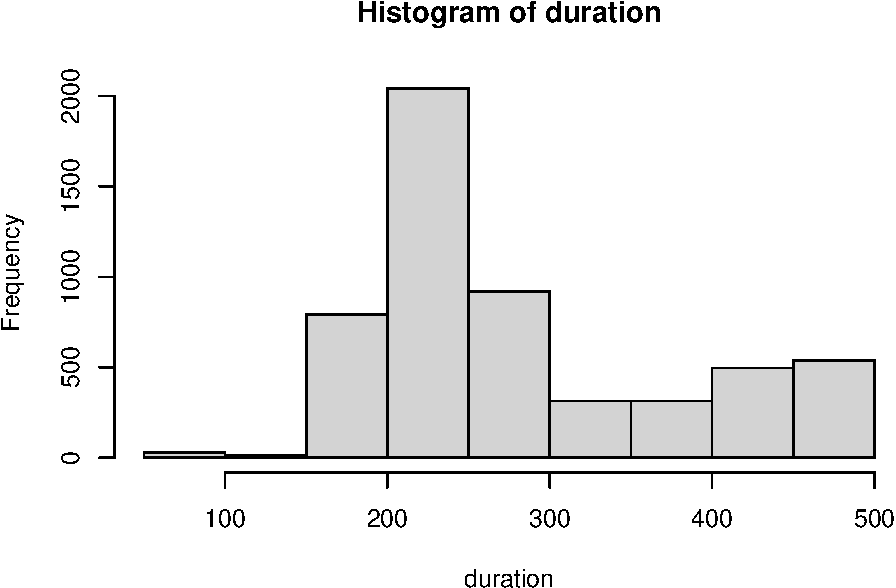
\includegraphics{code4stem_files/figure-latex/make histogram-1.pdf}

\begin{verbatim}
## $breaks
##  [1]  50 100 150 200 250 300 350 400 450 500
## 
## $counts
## [1]   28   15  792 2042  920  314  314  497  538
## 
## $density
## [1] 1.025641e-04 5.494505e-05 2.901099e-03 7.479853e-03 3.369963e-03
## [6] 1.150183e-03 1.150183e-03 1.820513e-03 1.970696e-03
## 
## $mids
## [1]  75 125 175 225 275 325 375 425 475
## 
## $xname
## [1] "duration"
## 
## $equidist
## [1] TRUE
## 
## attr(,"class")
## [1] "histogram"
\end{verbatim}

Computations by groups
Compute the mean duration for every start\_station:

\begin{Shaded}
\begin{Highlighting}[]
\NormalTok{mean_start_stn <-}\StringTok{ }\NormalTok{batrips[, .(}\DataTypeTok{mean_duration =} \KeywordTok{mean}\NormalTok{(duration)), by =}\StringTok{ }\NormalTok{start_station]}
\NormalTok{mean_start_stn }\OperatorTok
\StringTok{  }\KeywordTok{head}\NormalTok{(}\DecValTok{2}\NormalTok{)}
\end{Highlighting}
\end{Shaded}

\begin{verbatim}
##              start_station mean_duration
## 1: San Francisco City Hall      1893.936
## 2:  Embarcadero at Sansome      1418.182
\end{verbatim}

Compute the mean duration for every start and end station:

\begin{Shaded}
\begin{Highlighting}[]
\NormalTok{mean_station <-}\StringTok{ }\NormalTok{batrips[, .(}\DataTypeTok{mean_duration =} \KeywordTok{mean}\NormalTok{(duration)), by =}\StringTok{ }\NormalTok{.(start_station, end_station)]}
\NormalTok{mean_station }\OperatorTok
\StringTok{  }\KeywordTok{head}\NormalTok{(}\DecValTok{2}\NormalTok{)}
\end{Highlighting}
\end{Shaded}

\begin{verbatim}
##              start_station     end_station mean_duration
## 1: San Francisco City Hall Townsend at 7th      678.6364
## 2:  Embarcadero at Sansome Beale at Market      651.2367
\end{verbatim}

Compute the mean duration grouped by start\_station and month:

\begin{Shaded}
\begin{Highlighting}[]
\NormalTok{mean_start_station <-}\StringTok{ }\NormalTok{batrips[, .(}\DataTypeTok{mean_duration =} \KeywordTok{mean}\NormalTok{(duration)), by =}\StringTok{ }\NormalTok{.(start_station, }\KeywordTok{month}\NormalTok{(start_date))]}
\NormalTok{mean_start_station }\OperatorTok
\StringTok{  }\KeywordTok{head}\NormalTok{(}\DecValTok{2}\NormalTok{)}
\end{Highlighting}
\end{Shaded}

\begin{verbatim}
##              start_station month mean_duration
## 1: San Francisco City Hall     1     1548.2591
## 2:  Embarcadero at Sansome     1      952.1756
\end{verbatim}

Compute mean of duration and total trips grouped by start and end stations:

\begin{Shaded}
\begin{Highlighting}[]
\NormalTok{aggregate_mean_trips <-}\StringTok{ }\NormalTok{batrips[, .(}\DataTypeTok{mean_duration =} \KeywordTok{mean}\NormalTok{(duration), }
                                    \DataTypeTok{total_trips =}\NormalTok{ .N), }
\NormalTok{                                by =}\StringTok{ }\NormalTok{.(start_station, end_station)]}
\NormalTok{aggregate_mean_trips }\OperatorTok
\StringTok{  }\KeywordTok{head}\NormalTok{(}\DecValTok{2}\NormalTok{)}
\end{Highlighting}
\end{Shaded}

\begin{verbatim}
##              start_station     end_station mean_duration total_trips
## 1: San Francisco City Hall Townsend at 7th      678.6364         121
## 2:  Embarcadero at Sansome Beale at Market      651.2367         545
\end{verbatim}

Compute min and max duration grouped by start station, end station, and month:

\begin{Shaded}
\begin{Highlighting}[]
\NormalTok{aggregate_min_max <-}\StringTok{ }\NormalTok{batrips[, .(}\DataTypeTok{min_duration =} \KeywordTok{min}\NormalTok{(duration), }
                                 \DataTypeTok{max_duration =} \KeywordTok{max}\NormalTok{(duration)), }
\NormalTok{                             by =}\StringTok{ }\NormalTok{.(start_station, end_station, }
                                    \KeywordTok{month}\NormalTok{(start_date))]}
\NormalTok{aggregate_min_max }\OperatorTok
\StringTok{  }\KeywordTok{head}\NormalTok{(}\DecValTok{2}\NormalTok{)}
\end{Highlighting}
\end{Shaded}

\begin{verbatim}
##              start_station     end_station month min_duration max_duration
## 1: San Francisco City Hall Townsend at 7th     1          370          661
## 2:  Embarcadero at Sansome Beale at Market     1          345         1674
\end{verbatim}

Chaining data.table expressions:
Compute the total trips grouped by start\_station and end\_station

\begin{Shaded}
\begin{Highlighting}[]
\NormalTok{trips_dec <-}\StringTok{ }\NormalTok{batrips[, .N, by =}\StringTok{ }\NormalTok{.(start_station, }
\NormalTok{                                  end_station)]}
\NormalTok{trips_dec }\OperatorTok
\StringTok{  }\KeywordTok{head}\NormalTok{(}\DecValTok{2}\NormalTok{)}
\end{Highlighting}
\end{Shaded}

\begin{verbatim}
##              start_station     end_station   N
## 1: San Francisco City Hall Townsend at 7th 121
## 2:  Embarcadero at Sansome Beale at Market 545
\end{verbatim}

Arrange the total trips grouped by start\_station and end\_station in decreasing order:

\begin{Shaded}
\begin{Highlighting}[]
\NormalTok{trips_dec <-}\StringTok{ }\NormalTok{batrips[, .N, by =}\StringTok{ }\NormalTok{.(start_station, }
\NormalTok{                                  end_station)][}\KeywordTok{order}\NormalTok{(}\OperatorTok{-}\NormalTok{N)]}
\NormalTok{trips_dec }\OperatorTok
\StringTok{  }\KeywordTok{head}\NormalTok{(}\DecValTok{2}\NormalTok{)}
\end{Highlighting}
\end{Shaded}

\begin{verbatim}
##                              start_station
## 1:                         Townsend at 7th
## 2: San Francisco Caltrain 2 (330 Townsend)
##                                 end_station    N
## 1: San Francisco Caltrain (Townsend at 4th) 3158
## 2:                          Townsend at 7th 2937
\end{verbatim}

Top five most popular destinations:

\begin{Shaded}
\begin{Highlighting}[]
\NormalTok{top_}\DecValTok{5}\NormalTok{ <-}\StringTok{ }\NormalTok{batrips[, .N, by =}\StringTok{ }\NormalTok{end_station][}\KeywordTok{order}\NormalTok{(}\OperatorTok{-}\NormalTok{N)][}\DecValTok{1}\OperatorTok{:}\DecValTok{5}\NormalTok{]}
\NormalTok{top_}\DecValTok{5}
\end{Highlighting}
\end{Shaded}

\begin{verbatim}
##                                 end_station     N
## 1: San Francisco Caltrain (Townsend at 4th) 33213
## 2:     Harry Bridges Plaza (Ferry Building) 15692
## 3:  San Francisco Caltrain 2 (330 Townsend) 15333
## 4:                        Market at Sansome 14816
## 5:                          2nd at Townsend 14064
\end{verbatim}

Compute most popular end station for every start station:

\begin{Shaded}
\begin{Highlighting}[]
\NormalTok{popular_end_station <-}\StringTok{ }\NormalTok{trips_dec[, .(}\DataTypeTok{end_station =}\NormalTok{ end_station[}\DecValTok{1}\NormalTok{]), }
\NormalTok{                                 by =}\StringTok{ }\NormalTok{start_station]}
\NormalTok{popular_end_station }\OperatorTok
\StringTok{  }\KeywordTok{head}\NormalTok{(}\DecValTok{2}\NormalTok{)}
\end{Highlighting}
\end{Shaded}

\begin{verbatim}
##                              start_station
## 1:                         Townsend at 7th
## 2: San Francisco Caltrain 2 (330 Townsend)
##                                 end_station
## 1: San Francisco Caltrain (Townsend at 4th)
## 2:                          Townsend at 7th
\end{verbatim}

Find the first and last ride for each start\_station:

\begin{Shaded}
\begin{Highlighting}[]
\NormalTok{first_last <-}\StringTok{ }\NormalTok{batrips[}\KeywordTok{order}\NormalTok{(start_date), }
\NormalTok{                      .(}\DataTypeTok{start_date =}\NormalTok{ start_date[}\KeywordTok{c}\NormalTok{(}\DecValTok{1}\NormalTok{, .N)]), }
\NormalTok{                      by =}\StringTok{ }\NormalTok{start_station]}
\NormalTok{first_last}
\end{Highlighting}
\end{Shaded}

\begin{verbatim}
##                        start_station          start_date
##   1:         San Francisco City Hall 2014-01-01 00:14:00
##   2:         San Francisco City Hall 2014-12-31 22:06:00
##   3:          Embarcadero at Sansome 2014-01-01 00:17:00
##   4:          Embarcadero at Sansome 2014-12-31 22:08:00
##   5:               Steuart at Market 2014-01-01 00:23:00
##  ---                                                    
## 144: Santa Clara County Civic Center 2014-12-31 15:32:00
## 145:                     Ryland Park 2014-04-10 09:10:00
## 146:                     Ryland Park 2014-12-31 07:56:00
## 147:        Stanford in Redwood City 2014-09-03 19:41:00
## 148:        Stanford in Redwood City 2014-12-22 16:56:00
\end{verbatim}

Using .SD (I)

\begin{Shaded}
\begin{Highlighting}[]
\NormalTok{relevant_cols <-}\StringTok{ }\KeywordTok{c}\NormalTok{(}\StringTok{"start_station"}\NormalTok{, }\StringTok{"end_station"}\NormalTok{, }
                   \StringTok{"start_date"}\NormalTok{, }\StringTok{"end_date"}\NormalTok{, }\StringTok{"duration"}\NormalTok{)}
\end{Highlighting}
\end{Shaded}

Find the row corresponding to the shortest trip per month:

\begin{Shaded}
\begin{Highlighting}[]
\NormalTok{shortest <-}\StringTok{ }\NormalTok{batrips[, .SD[}\KeywordTok{which.min}\NormalTok{(duration)], }
\NormalTok{                    by =}\StringTok{ }\KeywordTok{month}\NormalTok{(start_date), }
\NormalTok{                    .SDcols =}\StringTok{ }\NormalTok{relevant_cols]}
\NormalTok{shortest }\OperatorTok
\StringTok{  }\KeywordTok{head}\NormalTok{(}\DecValTok{2}\NormalTok{)}
\end{Highlighting}
\end{Shaded}

\begin{verbatim}
##    month                            start_station
## 1:     1                          2nd at Townsend
## 2:     2 San Francisco Caltrain (Townsend at 4th)
##                                 end_station          start_date
## 1:                          2nd at Townsend 2014-01-21 13:01:00
## 2: San Francisco Caltrain (Townsend at 4th) 2014-02-08 14:28:00
##               end_date duration
## 1: 2014-01-21 13:02:00       60
## 2: 2014-02-08 14:29:00       61
\end{verbatim}

Using .SD (II)
Find the total number of unique start stations and zip codes per month:

\begin{Shaded}
\begin{Highlighting}[]
\NormalTok{unique_station_month <-}\StringTok{ }\NormalTok{batrips[, }\KeywordTok{lapply}\NormalTok{(.SD, uniqueN), }
\NormalTok{                                by =}\StringTok{ }\KeywordTok{month}\NormalTok{(start_date), }
\NormalTok{                                .SDcols =}\StringTok{ }\KeywordTok{c}\NormalTok{(}\StringTok{"start_station"}\NormalTok{, }\StringTok{"zip_code"}\NormalTok{)]}
\NormalTok{unique_station_month }\OperatorTok
\StringTok{  }\KeywordTok{head}\NormalTok{(}\DecValTok{2}\NormalTok{)}
\end{Highlighting}
\end{Shaded}

\begin{verbatim}
##    month start_station zip_code
## 1:     1            68      710
## 2:     2            69      591
\end{verbatim}

Adding and updating columns by reference
Add a new column, duration\_hour:

\begin{Shaded}
\begin{Highlighting}[]
\NormalTok{batrips[, duration_hour }\OperatorTok{:}\ErrorTok{=}\StringTok{ }\NormalTok{duration }\OperatorTok{/}\StringTok{ }\DecValTok{3600}\NormalTok{]}
\end{Highlighting}
\end{Shaded}

Fix/edit spelling in the second row of start\_station:

\begin{Shaded}
\begin{Highlighting}[]
\NormalTok{batrips[}\DecValTok{2}\NormalTok{, start_station }\OperatorTok{:}\ErrorTok{=}\StringTok{ "San Francisco City Hall 2"}\NormalTok{]}
\end{Highlighting}
\end{Shaded}

Replace negative duration values with NA:

\begin{Shaded}
\begin{Highlighting}[]
\NormalTok{batrips[duration }\OperatorTok{<}\StringTok{ }\DecValTok{0}\NormalTok{, duration }\OperatorTok{:}\ErrorTok{=}\StringTok{ }\OtherTok{NA}\NormalTok{]}
\end{Highlighting}
\end{Shaded}

Add a new column equal to total trips for every start station:

\begin{Shaded}
\begin{Highlighting}[]
\NormalTok{batrips[, trips_N }\OperatorTok{:}\ErrorTok{=}\StringTok{ }\NormalTok{.N, by =}\StringTok{ }\NormalTok{start_station]}
\end{Highlighting}
\end{Shaded}

Add new column for every start\_station and end\_station:

\begin{Shaded}
\begin{Highlighting}[]
\NormalTok{batrips[, duration_mean }\OperatorTok{:}\ErrorTok{=}\StringTok{ }\KeywordTok{mean}\NormalTok{(duration), by =}\StringTok{ }\NormalTok{.(start_station, end_station)]}
\end{Highlighting}
\end{Shaded}

Calculate the mean duration for each month:

\begin{Shaded}
\begin{Highlighting}[]
\NormalTok{batrips[, mean_dur }\OperatorTok{:}\ErrorTok{=}\StringTok{ }\KeywordTok{mean}\NormalTok{(duration, }\DataTypeTok{na.rm =} \OtherTok{TRUE}\NormalTok{), }
\NormalTok{            by =}\StringTok{ }\KeywordTok{month}\NormalTok{(start_date)]}
\end{Highlighting}
\end{Shaded}

Replace NA values in duration with the mean value of duration for that month:

\begin{Shaded}
\begin{Highlighting}[]
\NormalTok{batrips[, mean_dur }\OperatorTok{:}\ErrorTok{=}\StringTok{ }\KeywordTok{mean}\NormalTok{(duration, }\DataTypeTok{na.rm =} \OtherTok{TRUE}\NormalTok{), }
\NormalTok{            by =}\StringTok{ }\KeywordTok{month}\NormalTok{(start_date)][}\KeywordTok{is.na}\NormalTok{(duration), }
\NormalTok{                                    duration }\OperatorTok{:}\ErrorTok{=}\StringTok{ }\NormalTok{mean_dur]}
\end{Highlighting}
\end{Shaded}

Delete the mean\_dur column by reference:

\begin{Shaded}
\begin{Highlighting}[]
\NormalTok{batrips[, mean_dur }\OperatorTok{:}\ErrorTok{=}\StringTok{ }\KeywordTok{mean}\NormalTok{(duration, }\DataTypeTok{na.rm =} \OtherTok{TRUE}\NormalTok{), }
\NormalTok{            by =}\StringTok{ }\KeywordTok{month}\NormalTok{(start_date)][}\KeywordTok{is.na}\NormalTok{(duration), }
\NormalTok{                                    duration }\OperatorTok{:}\ErrorTok{=}\StringTok{ }\NormalTok{mean_dur][, mean_dur }\OperatorTok{:}\ErrorTok{=}\StringTok{ }\OtherTok{NULL}\NormalTok{]}
\end{Highlighting}
\end{Shaded}

Add columns using the LHS := RHS form
LHS := RHS form. In the LHS, you specify column names as a character vector and in the RHS, you specify values/expressions to be added inside list() (or the alias, .()):

\begin{Shaded}
\begin{Highlighting}[]
\NormalTok{batrips[, }\KeywordTok{c}\NormalTok{(}\StringTok{"mean_duration"}\NormalTok{, }
            \StringTok{"median_duration"}\NormalTok{) }\OperatorTok{:}\ErrorTok{=}\StringTok{ }\NormalTok{.(}\KeywordTok{mean}\NormalTok{(duration), }\KeywordTok{median}\NormalTok{(duration)), }
\NormalTok{        by =}\StringTok{ }\NormalTok{start_station]}
\end{Highlighting}
\end{Shaded}

Add columns using the functional form:

\begin{Shaded}
\begin{Highlighting}[]
\NormalTok{batrips[, }\StringTok{`}\DataTypeTok{:=}\StringTok{`}\NormalTok{(}\DataTypeTok{mean_duration =} \KeywordTok{mean}\NormalTok{(duration), }
               \DataTypeTok{median_duration =} \KeywordTok{median}\NormalTok{(duration)), }
\NormalTok{        by =}\StringTok{ }\NormalTok{start_station]}
\end{Highlighting}
\end{Shaded}

Add the mean\_duration column:

\begin{Shaded}
\begin{Highlighting}[]
\NormalTok{batrips[duration }\OperatorTok{>}\StringTok{ }\DecValTok{600}\NormalTok{, mean_duration }\OperatorTok{:}\ErrorTok{=}\StringTok{ }\KeywordTok{mean}\NormalTok{(duration), }
\NormalTok{        by =}\StringTok{ }\NormalTok{.(start_station, end_station)]}
\end{Highlighting}
\end{Shaded}

Use read.csv() to import batrips
Fread is much faster!

\begin{itemize}
\tightlist
\item
  system.time(read.csv(``batrips.csv''))
\item
  system.time(fread(``batrips.csv''))
\end{itemize}

Import using read.csv():

\begin{Shaded}
\begin{Highlighting}[]
\NormalTok{csv_file <-}\StringTok{ }\KeywordTok{read.csv}\NormalTok{(}\StringTok{"data/sample.csv"}\NormalTok{, }\DataTypeTok{fill =} \OtherTok{NA}\NormalTok{, }\DataTypeTok{quote =} \StringTok{""}\NormalTok{, }
                     \DataTypeTok{stringsAsFactors =} \OtherTok{FALSE}\NormalTok{, }\DataTypeTok{strip.white =} \OtherTok{TRUE}\NormalTok{, }
                     \DataTypeTok{header =} \OtherTok{TRUE}\NormalTok{)}
\NormalTok{csv_file }\OperatorTok
\StringTok{  }\KeywordTok{head}\NormalTok{(}\DecValTok{2}\NormalTok{)}
\end{Highlighting}
\end{Shaded}

\begin{verbatim}
##   YEAR    GEO Age_group  Sex                                     Element
## 1 1980 Canada         0 Both           Number of survivors at age x (lx)
## 2 1980 Canada         0 Both Number of deaths between age x and x+1 (dx)
##   AVG_VALUE
## 1    100000
## 2       976
\end{verbatim}

Import using fread():

\begin{Shaded}
\begin{Highlighting}[]
\NormalTok{csv_file <-}\StringTok{ }\KeywordTok{fread}\NormalTok{(}\StringTok{"data/sample.csv"}\NormalTok{)}
\NormalTok{csv_file }\OperatorTok
\StringTok{  }\KeywordTok{head}\NormalTok{(}\DecValTok{2}\NormalTok{)}
\end{Highlighting}
\end{Shaded}

\begin{verbatim}
##    YEAR    GEO Age_group  Sex                                     Element
## 1: 1980 Canada         0 Both           Number of survivors at age x (lx)
## 2: 1980 Canada         0 Both Number of deaths between age x and x+1 (dx)
##    AVG_VALUE
## 1:    100000
## 2:       976
\end{verbatim}

Check the class of Sex column:

\begin{Shaded}
\begin{Highlighting}[]
\KeywordTok{class}\NormalTok{(csv_file}\OperatorTok{$}\NormalTok{Sex)}
\end{Highlighting}
\end{Shaded}

\begin{verbatim}
## [1] "character"
\end{verbatim}

Import using read.csv with defaults:

\begin{Shaded}
\begin{Highlighting}[]
\KeywordTok{str}\NormalTok{(csv_file)}
\end{Highlighting}
\end{Shaded}

\begin{verbatim}
## Classes 'data.table' and 'data.frame':	1048575 obs. of  6 variables:
##  $ YEAR     : int  1980 1980 1980 1980 1980 1980 1980 1980 1980 1980 ...
##  $ GEO      : chr  "Canada" "Canada" "Canada" "Canada" ...
##  $ Age_group: int  0 0 0 0 0 0 0 0 0 0 ...
##  $ Sex      : chr  "Both" "Both" "Both" "Both" ...
##  $ Element  : chr  "Number of survivors at age x (lx)" "Number of deaths between age x and x+1 (dx)" "Death probability between age x and x+1 (qx)" "Margin of error of the death probability (m.e.(qx))" ...
##  $ AVG_VALUE: num  1.00e+05 9.76e+02 9.76e-03 1.80e-04 9.90e-01 ...
##  - attr(*, ".internal.selfref")=<externalptr>
\end{verbatim}

Select ``id'' and ``val'' columns:

\begin{Shaded}
\begin{Highlighting}[]
\NormalTok{select_columns <-}\StringTok{ }\KeywordTok{fread}\NormalTok{(}\StringTok{"data/sample.csv"}\NormalTok{, }\DataTypeTok{select =} \KeywordTok{c}\NormalTok{(}\StringTok{"GEO"}\NormalTok{, }\StringTok{"Sex"}\NormalTok{))}
\NormalTok{select_columns }\OperatorTok
\StringTok{  }\KeywordTok{head}\NormalTok{(}\DecValTok{2}\NormalTok{)}
\end{Highlighting}
\end{Shaded}

\begin{verbatim}
##       GEO  Sex
## 1: Canada Both
## 2: Canada Both
\end{verbatim}

Drop the ``val'' column:

\begin{Shaded}
\begin{Highlighting}[]
\NormalTok{drop_column <-}\StringTok{ }\KeywordTok{fread}\NormalTok{(}\StringTok{"data/sample.csv"}\NormalTok{, }\DataTypeTok{drop =} \StringTok{"Sex"}\NormalTok{)}
\NormalTok{drop_column }\OperatorTok
\StringTok{  }\KeywordTok{head}\NormalTok{(}\DecValTok{2}\NormalTok{)}
\end{Highlighting}
\end{Shaded}

\begin{verbatim}
##    YEAR    GEO Age_group                                     Element AVG_VALUE
## 1: 1980 Canada         0           Number of survivors at age x (lx)    100000
## 2: 1980 Canada         0 Number of deaths between age x and x+1 (dx)       976
\end{verbatim}

Import the file while avoiding the warning:

\begin{Shaded}
\begin{Highlighting}[]
\NormalTok{only_data <-}\StringTok{ }\KeywordTok{fread}\NormalTok{(}\StringTok{"data/sample.csv"}\NormalTok{, }\DataTypeTok{nrows =} \DecValTok{3}\NormalTok{)}
\NormalTok{only_data}
\end{Highlighting}
\end{Shaded}

\begin{verbatim}
##    YEAR    GEO Age_group  Sex                                      Element
## 1: 1980 Canada         0 Both            Number of survivors at age x (lx)
## 2: 1980 Canada         0 Both  Number of deaths between age x and x+1 (dx)
## 3: 1980 Canada         0 Both Death probability between age x and x+1 (qx)
##    AVG_VALUE
## 1:  1.00e+05
## 2:  9.76e+02
## 3:  9.76e-03
\end{verbatim}

Import only the metadata:

\begin{Shaded}
\begin{Highlighting}[]
\NormalTok{only_metadata <-}\StringTok{ }\KeywordTok{fread}\NormalTok{(}\StringTok{"data/sample.csv"}\NormalTok{, }\DataTypeTok{skip =} \DecValTok{7}\NormalTok{)}
\NormalTok{only_metadata }\OperatorTok
\StringTok{  }\KeywordTok{head}\NormalTok{(}\DecValTok{2}\NormalTok{)}
\end{Highlighting}
\end{Shaded}

\begin{verbatim}
##      V1     V2 V3   V4                                                      V5
## 1: 1980 Canada  0 Both Cumulative number of life years lived beyond age x (Tx)
## 2: 1980 Canada  0 Both                Life expectancy (in years) at age x (ex)
##           V6
## 1: 7543058.0
## 2:      75.4
\end{verbatim}

Import using read.csv:

\begin{Shaded}
\begin{Highlighting}[]
\NormalTok{base_r <-}\StringTok{ }\KeywordTok{read.csv}\NormalTok{(}\StringTok{"data/sample.csv"}\NormalTok{, }
                   \DataTypeTok{colClasses =} \KeywordTok{c}\NormalTok{(}\KeywordTok{rep}\NormalTok{(}\StringTok{"factor"}\NormalTok{, }\DecValTok{4}\NormalTok{), }
                                  \StringTok{"character"}\NormalTok{, }
                                  \StringTok{"numeric"}\NormalTok{))}
\KeywordTok{str}\NormalTok{(base_r)}
\end{Highlighting}
\end{Shaded}

\begin{verbatim}
## 'data.frame':	1048575 obs. of  6 variables:
##  $ YEAR     : Factor w/ 35 levels "1980","1981",..: 1 1 1 1 1 1 1 1 1 1 ...
##  $ GEO      : Factor w/ 10 levels "Alberta","British Columbia",..: 3 3 3 3 3 3 3 3 3 3 ...
##  $ Age_group: Factor w/ 111 levels "0","1","10","100",..: 1 1 1 1 1 1 1 1 1 1 ...
##  $ Sex      : Factor w/ 3 levels "Both","F","M": 1 1 1 1 1 1 1 1 1 3 ...
##  $ Element  : chr  "Number of survivors at age x (lx)" "Number of deaths between age x and x+1 (dx)" "Death probability between age x and x+1 (qx)" "Margin of error of the death probability (m.e.(qx))" ...
##  $ AVG_VALUE: num  1.00e+05 9.76e+02 9.76e-03 1.80e-04 9.90e-01 ...
\end{verbatim}

Import using fread:

\begin{Shaded}
\begin{Highlighting}[]
\NormalTok{import_fread <-}\StringTok{ }\KeywordTok{fread}\NormalTok{(}\StringTok{"data/sample.csv"}\NormalTok{, }
                      \DataTypeTok{colClasses =} \KeywordTok{list}\NormalTok{(}\DataTypeTok{factor =} \DecValTok{1}\OperatorTok{:}\DecValTok{4}\NormalTok{, }\DataTypeTok{numeric =} \DecValTok{7}\OperatorTok{:}\DecValTok{10}\NormalTok{))}
\end{Highlighting}
\end{Shaded}

\begin{verbatim}
## Warning in fread("data/sample.csv", colClasses = list(factor = 1:4, numeric =
## 7:10)): Column number 7 (colClasses[[2]][1]) is out of range [1,ncol=6]
\end{verbatim}

\begin{verbatim}
## Warning in fread("data/sample.csv", colClasses = list(factor = 1:4, numeric =
## 7:10)): Column number 8 (colClasses[[2]][2]) is out of range [1,ncol=6]
\end{verbatim}

\begin{verbatim}
## Warning in fread("data/sample.csv", colClasses = list(factor = 1:4, numeric =
## 7:10)): Column number 9 (colClasses[[2]][3]) is out of range [1,ncol=6]
\end{verbatim}

\begin{verbatim}
## Warning in fread("data/sample.csv", colClasses = list(factor = 1:4, numeric =
## 7:10)): Column number 10 (colClasses[[2]][4]) is out of range [1,ncol=6]
\end{verbatim}

\begin{Shaded}
\begin{Highlighting}[]
\KeywordTok{str}\NormalTok{(import_fread)}
\end{Highlighting}
\end{Shaded}

\begin{verbatim}
## Classes 'data.table' and 'data.frame':	1048575 obs. of  6 variables:
##  $ YEAR     : Factor w/ 35 levels "1980","1981",..: 1 1 1 1 1 1 1 1 1 1 ...
##  $ GEO      : Factor w/ 10 levels "Alberta","British Columbia",..: 3 3 3 3 3 3 3 3 3 3 ...
##  $ Age_group: Factor w/ 111 levels "0","1","10","100",..: 1 1 1 1 1 1 1 1 1 1 ...
##  $ Sex      : Factor w/ 3 levels "Both","F","M": 1 1 1 1 1 1 1 1 1 3 ...
##  $ Element  : chr  "Number of survivors at age x (lx)" "Number of deaths between age x and x+1 (dx)" "Death probability between age x and x+1 (qx)" "Margin of error of the death probability (m.e.(qx))" ...
##  $ AVG_VALUE: num  1.00e+05 9.76e+02 9.76e-03 1.80e-04 9.90e-01 ...
##  - attr(*, ".internal.selfref")=<externalptr>
\end{verbatim}

Import the file correctly, use the fill argument to ensure all rows are imported correctly:

\begin{Shaded}
\begin{Highlighting}[]
\NormalTok{correct <-}\StringTok{ }\KeywordTok{fread}\NormalTok{(}\StringTok{"data/sample.csv"}\NormalTok{, }\DataTypeTok{fill =} \OtherTok{TRUE}\NormalTok{)}
\NormalTok{correct }\OperatorTok
\StringTok{  }\KeywordTok{head}\NormalTok{(}\DecValTok{2}\NormalTok{)}
\end{Highlighting}
\end{Shaded}

\begin{verbatim}
##    YEAR    GEO Age_group  Sex                                     Element
## 1: 1980 Canada         0 Both           Number of survivors at age x (lx)
## 2: 1980 Canada         0 Both Number of deaths between age x and x+1 (dx)
##    AVG_VALUE
## 1:    100000
## 2:       976
\end{verbatim}

Import the file using na.strings
The missing values are encoded as ``\#\#''. Note that fread() handles an empty field ,, by default as NA

\begin{Shaded}
\begin{Highlighting}[]
\NormalTok{missing_values <-}\StringTok{ }\KeywordTok{fread}\NormalTok{(}\StringTok{"data/sample.csv"}\NormalTok{, }\DataTypeTok{na.strings =} \StringTok{"##"}\NormalTok{) }
\NormalTok{missing_values }\OperatorTok
\StringTok{  }\KeywordTok{head}\NormalTok{(}\DecValTok{2}\NormalTok{)}
\end{Highlighting}
\end{Shaded}

\begin{verbatim}
##    YEAR    GEO Age_group  Sex                                     Element
## 1: 1980 Canada         0 Both           Number of survivors at age x (lx)
## 2: 1980 Canada         0 Both Number of deaths between age x and x+1 (dx)
##    AVG_VALUE
## 1:  1.00E+05
## 2:       976
\end{verbatim}

Write dt to fwrite.txt:
- fwrite(dt, ``fwrite.txt'')

Import the file using readLines():

\begin{Shaded}
\begin{Highlighting}[]
\KeywordTok{readLines}\NormalTok{(}\StringTok{"data/sample.csv"}\NormalTok{) }\OperatorTok
\StringTok{  }\KeywordTok{head}\NormalTok{(}\DecValTok{2}\NormalTok{)}
\end{Highlighting}
\end{Shaded}

\begin{verbatim}
## Warning in readLines("data/sample.csv"): incomplete final line found on 'data/
## sample.csv'
\end{verbatim}

\begin{verbatim}
## [1] "YEAR,GEO,Age_group,Sex,Element,AVG_VALUE"                     
## [2] "1980,Canada,0,Both,Number of survivors at age x (lx),1.00E+05"
\end{verbatim}

Write batrips\_dates to file using ``ISO'' format:
- fwrite(batrips\_dates, ``iso.txt'', dateTimeAs = ``ISO'')

Write batrips\_dates to file using ``squash'' format:
- fwrite(batrips\_dates, ``squash.txt'', dateTimeAs = ``squash'')

\begin{center}\rule{0.5\linewidth}{0.5pt}\end{center}

\hypertarget{beginner-resources-by-topic}{%
\section{Beginner Resources by Topic}\label{beginner-resources-by-topic}}

\begin{center}\rule{0.5\linewidth}{0.5pt}\end{center}

\hypertarget{getting-set-up-with-r-rstudio}{%
\subsection{Getting Set-Up with R \& RStudio}\label{getting-set-up-with-r-rstudio}}

\begin{itemize}
\tightlist
\item
  \textbf{Download \& Install R:}

  \begin{itemize}
  \tightlist
  \item
    \url{https://cran.r-project.org}
  \item
    For Mac: click on \textbf{Download R for (Mac) OS X}, look at the top link under \textbf{Files}, which at time of writing is \textbf{R-3.2.4.pkg}, and download this if compatible with your current version mac OS (Mavericks 10.9 or higher). Otherwise download the version beneath it which is compatible for older mac OS versions. Then install the downloaded software.
  \item
    For Windows: click on \textbf{Download R for Windows}, then click on the link \textbf{install R for the first time}, and download from the large link at the top of the page which at time of writing is \textbf{Download R 3.2.4 for Windows}. Then install the downloaded software.
  \end{itemize}
\item
  \textbf{Download \& Install RStudio:}

  \begin{itemize}
  \tightlist
  \item
    \url{https://www.rstudio.com/products/rstudio/download/}
  \item
    For Mac: under the \textbf{Installers for Supported Platforms} heading click the link with \textbf{Mac OS X} in it. Install the downloaded software.
  \item
    For Windows: under the \textbf{Installers for Supported Platforms} heading click the link with \textbf{Windows Vista} in it. Install the downloaded software.
  \end{itemize}
\item
  \textbf{Exercises in R: swirl (HIGHLY RECOMMENDED):}

  \begin{itemize}
  \tightlist
  \item
    \url{http://swirlstats.com/students.html}
  \end{itemize}
\item
  \textbf{Data Prep}:

  \begin{itemize}
  \tightlist
  \item
    Intro to dplyr: \url{https://cran.rstudio.com/web/packages/dplyr/vignettes/introduction.html}
  \item
    Data Manipulation (detailed): \url{http://www.sr.bham.ac.uk/~ajrs/R/index.html}
  \item
    Aggregation and Restructing Data (base \& reshape): \url{http://www.r-statistics.com/2012/01/aggregation-and-restructuring-data-from-r-in-action/}
  \end{itemize}
\item
  \textbf{Data Types intro}: Vectors, Matrices, Arrays, Data Frames, Lists, Factors: \url{http://www.statmethods.net/input/datatypes.html}
\item
  \textbf{Using Dates and Times}: \url{http://www.cyclismo.org/tutorial/R/time.html}
\item
  \textbf{Text Data and Character Strings}: \url{http://gastonsanchez.com/Handling_and_Processing_Strings_in_R.pdf}
\item
  \textbf{Data Mining}: \url{http://www.rdatamining.com}
\end{itemize}

\begin{center}\rule{0.5\linewidth}{0.5pt}\end{center}

\begin{itemize}
\tightlist
\item
  \textbf{Data Viz}:

  \begin{itemize}
  \tightlist
  \item
    ggplot2 Cheat Sheet (RECOMMENDED): \url{http://zevross.com/blog/2014/08/04/beautiful-plotting-in-r-a-ggplot2-cheatsheet-3/}
  \item
    ggplot2 theoretical tutorial (detailed but RECOMMENDED): \url{http://www.ling.upenn.edu/~joseff/avml2012/}
  \item
    Examples of base R, ggplot2, and rCharts: \url{http://patilv.com/Replication-of-few-graphs-charts-in-base-R-ggplot2-and-rCharts-part-1-base-R/}
  \item
    Intro to ggplot2: \url{http://heather.cs.ucdavis.edu/~matloff/GGPlot2/GGPlot2Intro.pdf}
  \end{itemize}
\item
  \textbf{Interactive Visualisations}:

  \begin{itemize}
  \tightlist
  \item
    Interactive graphics (rCharts, jQuery): \url{http://www.computerworld.com/article/2473365/business-intelligence/business-intelligence-106897-how-to-turn-csv-data-into-interactive-visualizations-with-r-and-rchart.html}
  \end{itemize}
\end{itemize}

\begin{center}\rule{0.5\linewidth}{0.5pt}\end{center}

\begin{itemize}
\tightlist
\item
  \textbf{Statistics}:

  \begin{itemize}
  \tightlist
  \item
    Detailed Statistics Primer: \url{http://health.adelaide.edu.au/psychology/ccs/docs/lsr/lsr-0.3.pdf}
  \item
    Beginner guide to statistical topics in R: \url{http://www.cyclismo.org/tutorial/R/}
  \end{itemize}
\item
  \textbf{Linear Models}: \url{http://data.princeton.edu/R/gettingStarted.html}
\item
  \textbf{Time Series Analysis}: \url{https://www.otexts.org/fpp/resources}
\item
  \textbf{Little Book of R series}:

  \begin{itemize}
  \tightlist
  \item
    Time Series: \url{http://a-little-book-of-r-for-time-series.readthedocs.org/en/latest/}
  \item
    Biomedical Statistics: \url{http://a-little-book-of-r-for-biomedical-statistics.readthedocs.org/en/latest/}
  \item
    Multivariate Statistics: \url{http://little-book-of-r-for-multivariate-analysis.readthedocs.org/en/latest/}
  \end{itemize}
\end{itemize}

\begin{center}\rule{0.5\linewidth}{0.5pt}\end{center}

\begin{itemize}
\tightlist
\item
  \textbf{RStudio Cheat Sheets}:

  \begin{itemize}
  \tightlist
  \item
    RStudio IDE: \url{http://www.rstudio.com/wp-content/uploads/2016/01/rstudio-IDE-cheatsheet.pdf}
  \item
    Data Wrangling (dplyr \& tidyr): \url{https://www.rstudio.com/wp-content/uploads/2015/02/data-wrangling-cheatsheet.pdf}
  \item
    Data Viz (ggplot2): \url{https://www.rstudio.com/wp-content/uploads/2015/03/ggplot2-cheatsheet.pdf}
  \item
    Reproducible Reports (markdown): \url{https://www.rstudio.com/wp-content/uploads/2015/02/rmarkdown-cheatsheet.pdf}
  \item
    Interactive Web Apps (shiny): \url{https://www.rstudio.com/wp-content/uploads/2015/02/shiny-cheatsheet.pdf}
  \end{itemize}
\end{itemize}

\begin{center}\rule{0.5\linewidth}{0.5pt}\end{center}

\hypertarget{specialist-topics}{%
\subsection{Specialist Topics}\label{specialist-topics}}

\begin{itemize}
\tightlist
\item
  \textbf{Google Analytics}: \url{http://online-behavior.com/analytics/r}
\item
  \textbf{Spatial Cheat Sheet}: \url{http://www.maths.lancs.ac.uk/~rowlings/Teaching/UseR2012/cheatsheet.html}
\item
  \textbf{Translating between R and SQL}: \url{http://www.burns-stat.com/translating-r-sql-basics/}
\item
  \textbf{Google's R style guide}: \url{https://google.github.io/styleguide/Rguide.xml}
\end{itemize}

\begin{center}\rule{0.5\linewidth}{0.5pt}\end{center}

\hypertarget{operational-basics}{%
\subsection{Operational Basics}\label{operational-basics}}

\begin{itemize}
\tightlist
\item
  \textbf{Working Directory}:\\
  Example on a mac = \texttt{setwd("\textasciitilde{}/Desktop/R")} or \texttt{setwd("/Users/CRT/Desktop/R")}\\
  Example on windows = \texttt{setwd("C:/Desktop/R")}\\
\item
  \textbf{Help}:\\
  \texttt{?functionName}~\\
  \texttt{example(functionName)}~\\
  \texttt{args(functionName)}~\\
  \texttt{help.search("your\ search\ term")}~\\
\item
  \textbf{Assignment Operator}: \texttt{\textless{}-}
\end{itemize}

\begin{center}\rule{0.5\linewidth}{0.5pt}\end{center}

\hypertarget{getting-your-data-into-r}{%
\section{Getting Your Data into R}\label{getting-your-data-into-r}}

\begin{enumerate}
\def\labelenumi{\arabic{enumi}.}
\tightlist
\item
  Loading Existing Local Data
\end{enumerate}

\begin{enumerate}
\def\labelenumi{(\alph{enumi})}
\tightlist
\item
  When already in the working directory where the data is
\end{enumerate}

Import a local \textbf{csv} file (i.e.~where data is separated by \textbf{commas}), saving it as an object:

\begin{Shaded}
\begin{Highlighting}[]
\CommentTok{#this will create a data frame called "object"}
\CommentTok{#the header argument is defaulted to TRUE, i.e. read.csv assumes your file has a header row and will take the first row of your csv to be the column names}
\NormalTok{object <-}\StringTok{ }\KeywordTok{read.csv}\NormalTok{(}\StringTok{"xxx.csv"}\NormalTok{)}

\CommentTok{#if your csv does not have a header row, add header = FALSE to the command}
\CommentTok{#in this call default column headers will be assigned which can be changed}
\NormalTok{object <-}\StringTok{ }\KeywordTok{read.csv}\NormalTok{(}\StringTok{"xxx.csv"}\NormalTok{, }\DataTypeTok{header =} \OtherTok{FALSE}\NormalTok{)}
\end{Highlighting}
\end{Shaded}

Import a local tab delimited file (i.e.~where data is separated by \textbf{tabs}), saving is as an object:

\begin{enumerate}
\def\labelenumi{(\alph{enumi})}
\setcounter{enumi}{1}
\tightlist
\item
  When NOT in the working directory where the data is
\end{enumerate}

For example to import and save a local \textbf{csv} file from a different working directory you can either need to specify the file path (operating system specific), e.g.:

\begin{Shaded}
\begin{Highlighting}[]
\CommentTok{#on a mac}
\NormalTok{object <-}\StringTok{ }\KeywordTok{read.csv}\NormalTok{(}\StringTok{"~/Desktop/R/data.csv"}\NormalTok{)}

\CommentTok{#on windows}
\NormalTok{object <-}\StringTok{ }\KeywordTok{read.csv}\NormalTok{(}\StringTok{"C:/Desktop/R/data.csv"}\NormalTok{)}
\end{Highlighting}
\end{Shaded}

OR

You can use the file.choose() command which will interactively open up the file dialog box for you to browse and select the local file, e.g.:

\begin{Shaded}
\begin{Highlighting}[]
\NormalTok{object <-}\StringTok{ }\KeywordTok{read.csv}\NormalTok{(}\KeywordTok{file.choose}\NormalTok{())}
\end{Highlighting}
\end{Shaded}

\begin{enumerate}
\def\labelenumi{(\alph{enumi})}
\setcounter{enumi}{2}
\tightlist
\item
  Copying and Pasting Data
\end{enumerate}

For relatively small amounts of data you can do an equivalent copy paste (operating system specific):

\begin{Shaded}
\begin{Highlighting}[]
\CommentTok{#on a mac}
\NormalTok{object <-}\StringTok{ }\KeywordTok{read.table}\NormalTok{(}\KeywordTok{pipe}\NormalTok{(}\StringTok{"pbpaste"}\NormalTok{))}

\CommentTok{#on windows}
\NormalTok{object <-}\StringTok{ }\KeywordTok{read.table}\NormalTok{(}\DataTypeTok{file =} \StringTok{"clipboard"}\NormalTok{)}
\end{Highlighting}
\end{Shaded}

\begin{enumerate}
\def\labelenumi{\arabic{enumi}.}
\setcounter{enumi}{1}
\tightlist
\item
  Loading Non-Numerical Data - character strings
\end{enumerate}

Be careful when loading text data! R may assume character strings are statistical factor variables, e.g. ``low'', ``medium'', ``high'', when are just individual labels like names. To specify text data NOT to be converted into factor variables, add \texttt{stringsAsFactor\ =\ FALSE} to your \texttt{read.csv/read.table} command:

\begin{Shaded}
\begin{Highlighting}[]
\NormalTok{object <-}\StringTok{ }\KeywordTok{read.table}\NormalTok{(}\StringTok{"xxx.txt"}\NormalTok{, }\DataTypeTok{stringsAsFactors =} \OtherTok{FALSE}\NormalTok{)}
\end{Highlighting}
\end{Shaded}

\begin{enumerate}
\def\labelenumi{\arabic{enumi}.}
\setcounter{enumi}{2}
\tightlist
\item
  Downloading Remote Data
\end{enumerate}

For accessing files from the web you can use the same \texttt{read.csv/read.table} commands. However, the file being downloaded does need to be in an R-friendly format (maximum of 1 header row, subsequent rows are the equivalent of one data record per row, no extraneous footnotes etc.). Here is an example downloading an online csv file from Pew Research:

\begin{Shaded}
\begin{Highlighting}[]
\NormalTok{object <-}\StringTok{ }\KeywordTok{read.csv}\NormalTok{(}\StringTok{"https://vincentarelbundock.github.io/Rdatasets/csv/datasets/AirPassengers.csv"}\NormalTok{)}
\end{Highlighting}
\end{Shaded}

\begin{enumerate}
\def\labelenumi{\arabic{enumi}.}
\setcounter{enumi}{3}
\tightlist
\item
  Other Formats - Excel, SPSS, SAS etc.
\end{enumerate}

For other file formats, you will need specific R packages to import these data.

Here's a good site for an overview: \url{http://www.statmethods.net/input/importingdata.html}

Here's a more detailed site: \url{http://r4stats.com/examples/data-import/}

Here's some info on the \texttt{foreign} package for loading statistical software file types: \url{http://www.ats.ucla.edu/stat/r/faq/inputdata_R.htm}

\begin{center}\rule{0.5\linewidth}{0.5pt}\end{center}

\hypertarget{getting-your-data-out-of-r}{%
\section{Getting Your Data out of R}\label{getting-your-data-out-of-r}}

\begin{enumerate}
\def\labelenumi{\arabic{enumi}.}
\tightlist
\item
  Exporting data
\end{enumerate}

Navigate to the working directory you want to save the data table into, then run the command (in this case creating a tab delimited file):
- write.table(object, ``xxx.txt'', sep = "\t")

\begin{enumerate}
\def\labelenumi{\arabic{enumi}.}
\setcounter{enumi}{1}
\tightlist
\item
  Save down an R object
  Navigate to the working directory you want to save the object in then run the command:
\end{enumerate}

\begin{itemize}
\tightlist
\item
  save(object, file = ``xxx.rda'')
\end{itemize}

reload the object:
- load(``xxx.rda'')

\begin{center}\rule{0.5\linewidth}{0.5pt}\end{center}

\end{document}
